\documentclass[12pt]{book}
\usepackage{amsmath}
\usepackage{float}
\usepackage[margin=1.5in]{geometry}
\usepackage{enumitem}
\usepackage{xcolor}
\usepackage{cancel}
\usepackage{graphicx}



\title{Introduction to Mechanics}
\author{Nathan Butcher}

\begin{document}
\graphicspath{{Figures/Units} {Figures/Forces} {Figures/WorkEnergy} {Figures/Momentum} {Figures/Rotation} {Figures/SolarSystem}}
\newcounter{chp}
\setcounter{chp}{0}
\newcounter{example}

\newcommand{\scinot}[2]{#1 \cdot 10^{#2}}

%Start a new example using counters
\newcommand{\example}{\textbf{Example \texttt{\thechp}.\texttt{\theexample}}
\addtocounter{example}{1}

\hspace{10pt}
}

%Give a horizontal line with space to separte things
%like examples or asides
\newcommand{\linespace}{\hspace{10pt}

\hrule

\hspace{10pt}}

\newenvironment{exampleblock}
{
\linespace

\example

}
{

\linespace

}

\tableofcontents

\chapter{Introduction, Numbers, and Units}

\setcounter{example}{1}
\addtocounter{chp}{1}

In physics we study the interactions and motion of matter. For our introduction in this class, we will mostly study what I like to call ``Physics at the human scale'' because it is the physics of daily life that we observe and directly interact with. It describes an apple falling from a tree, a car slamming its brakes, a pendulum swinging, the collision of 2 billiard balls, and more.

\section{Math and Scientific Notation}

This text will assume that you are comfortable with using algebra to solve an equation for a variable and that you have had a class on trigonometry. We will review those topics as they come up but it may be difficult to follow without the math background.

During this text we will use \textbf{scientific notation} frequently to write very large or very small numbers in an easier to read format. With it, we write a number in the format

\begin{equation}
\scinot{a}{b}
\end{equation}

where $1 \leq a < 10$ and $b$ is an integer. This saves us from having to write and count a lot of zeros that indicate place. The number is a factor multiplied by a power of 10.

\begin{exampleblock}

Write the number 38,500,000 in scientific notation.

\hspace{10pt}

To write this in the form $\scinot{a}{b}$, first let's find $a$ such that $1 \leq a < 10$. Since our number starts with the digits 385, that means $a = 3.85$. From here we have

\begin{equation}
38,500,000 = 3.85 \cdot 10,000,000
\end{equation}

Now we need to write 10,000,000 as a power of 10. There are 7 zeros, so it will be $10^7$. This means that our number is 

\begin{equation}
\scinot{3.85}{7}
\end{equation}

\end{exampleblock}

\begin{exampleblock}

Write the number 0.000007018 in scientific notation.

\hspace{10pt}

We can use the same reasoning as the above example to find that $a = 7.018$. The number can be written as

\begin{equation}
0.000007018 = 7.018 \cdot 0.000001
\end{equation}

Now we just need to find the power of 10. Let's start looking at powers of 10.

\begin{equation}
\begin{split}
10^0 = 1 \\
10^{-1} = \frac{1}{10} = 0.1 \\
10^{-2} = \frac{1}{10^2} = 0.01 \\
10^{-3} = \frac{1}{10^3} = 0.001
\end{split}
\end{equation}

A negative power means to take 1 divided by the number to that positive power. Looking at 10, we see that as we decrease the power (larger negative value), we move the decimal point 1 to the left. This will give us

\begin{equation}
0.000001 = \frac{1}{10^6} = 10^{-6}
\end{equation}

which makes our number

\begin{equation}
0.000007018 = \scinot{7.018}{-6}
\end{equation}

\end{exampleblock}

\section{Units}

Physicists will try to describe the world around us quantitatively, meaning with numbers. In order to ascribe meaning to those numbers we need to use physical \textbf{units}. For example, think about if you were baking a loaf of bread and the recipe called for ``4 flour''. Would you know how much flour was required? The recipe should say ``4 \textit{cups} of flour'' so that you know the amount required for the bread. 

In physics, like most sciences, we use \textbf{SI units}. In the USA, you likely encounter the Imperial system of units in daily life. Common Imperial units you might have seen include the inch for length and gallon for volume. These units are not the standard for scientific disciplines, and as such we will focus on using SI units. There are 3 base units that we will use frequently:

\begin{itemize}
\item \textbf{kilogram} - the SI base unit of mass. Mass is a measure of how much matter there is. It is related to but not the same as weight. We will discuss weight further in a later chapter, but for now think of mass as how much ``stuff'' there is.

\item \textbf{meter} - the SI base unit of length. If you don't have a good mental picture of a meter, it is a little longer than 3 feet.

\item \textbf{second} - the SI base unit of time. We will continue to see minutes and hours used throughout, but for doing quantitative work we will want to use seconds for everything.
\end{itemize}

\section{SI Prefixes}

With these SI base units we use \textbf{prefixes} to scale the units relative to our problem. Table \ref{SIPrefixes} contains several of the most common prefixes, with the bolded ones being most important for this class.

\begin{table}[b]
\large
\centering
\caption{SI Prefixes}
\begin{tabular}{ c | c | c }
	\hline
	Prefix & Abbreviation & Numerical value \\
	\hline
	nano- & n & $10^{-9}$ \\
	micro- & $\mu$ (Greek letter \textit{mu}) & $10^{-6}$ \\
	\textbf{milli-} & m & $10^{-3}$ \\
	\textbf{centi-} & c & $10^{-2}$ \\
	\textbf{kilo-} & k & $10^3$ \\
	mega- & M & $10^6$ \\
	giga- & G & $10^9$ \\
	\hline
\end{tabular}

\label{SIPrefixes}
\end{table}

One thing you should see is that SI prefixes allow us to scale our units by powers of 10. This is much simpler than the Imperial system. For lengths we have 12 inches to a foot, 3 feet to a yard, and 1760 yards to a mile. Compare this to just multiplying or dividing by powers of 10 and see how much simpler SI units are to work with!

The main purpose to having the prefixes is it allows us to scale the units to our problem. If we were to talk about the distance between San Diego and Los Angeles, it would make sense to use kilometers because that distance is about 194 kilometers. In meters, it would be $194 \cdot 10^3 = 194,000$ meters. Prefixes allow us to use numbers that are closer to 1, which are easier to read and for our brains to process. 

There are other prefixes and units that are used within different branches of physics and other fields of science. We will see some of this in CHAPTER HERE when we discuss the solar system. Again, the goal is always to make the numbers we work with closer to 1.

In addition to the base units, we will also have \textbf{derived units}, which are a combination of SI base units. On a car speedometer you may have seen the unit $km/hr$, which means ``kilometers per hour''. This is a derived unit because it combines the units of length and time.


\section{Converting Units}

Now that we have SI prefixes, it is important that we learn how to convert between different units. This process is called \textbf{dimensional analysis} because the units are the ``dimensions'' that we are looking at.

To convert units, we will write unit factors that are fractions equal to 1. For example, 

\begin{equation}
\frac{1 \, mm}{10^{-3} \, m} = 1
\end{equation}

is a unit factor that equals 1 because the prefix milli- means $10^{-3}$, so 1 millimeter is equal to $10^{-3}$ meter. This fraction can by multiplied by a quantity to change the unit but not the physical value because the fraction is 1. Now lets use that to convert 3.25 meters to millimeters. We can use the unit fraction to cancel the meters from the original value, and have a unit of millimeters left in the numerator.

\begin{equation}
3.25 \, \cancel{m} \cdot \frac{1 \, mm}{10^{-3} \, \cancel{m}} = 3,250 \, mm
\end{equation}


The reason this works is that our unit fraction is equal to 1, so multiplying our original quantity by that unit fraction doesn't change the value! It only changes what unit that value is given in.

You could also think of the unit fraction as 1,000 millimeters in a meter.

\begin{equation}
3.25 \, \cancel{m} \cdot \frac{1000 \, mm}{1 \, \cancel{m}} = 3,250 \, mm
\end{equation}

Both $\frac{1000 \, mm}{1 \, m}$ and $\frac{1 \, mm}{10^{-3} \, m}$ are valid unit fractions for converting from meters to millieters. They are equally correct, so use whichever you prefer!

%\textbf{Example \texttt{\thechp}.\texttt{\theexample}}
%\addtocounter{example}{1}
\begin{exampleblock}

\textbf{Convert 500 nanometers to centimeters.}

\hspace{10pt}

We can convert 500 nanometers to meters first, then convert from meters to centimeters.

\begin{equation}
500 \, \cancel{nm} \cdot = \frac{10^{-9} \, m}{1 \, \cancel{nm}} = 5 \cdot 10^{-7} \, m
\end{equation}

\begin{equation}
\scinot{5}{-7} \, \cancel{m} = \frac{100 \, cm}{1 \, \cancel{m}} = \scinot{5}{-5} \, cm 
\end{equation}

Sometimes it is useful to convert to an intermediary unit to help you get to the requested final unit.
\end{exampleblock}

%\linespace

%\example

\begin{exampleblock}

Convert 1 meter to feet. Use the following information:

\begin{itemize}
\item 1 foot = 12 inches
\item 1 inch = 2.54 cm
\end{itemize}

The given unit conversions tell us how to solve this problem. First we convert the meter to centimeters, then use the given conversion from centimeters to inches. Finally, we can use the given conversion from inches to feet.

\begin{equation}
1 \, \cancel{m} \cdot \frac{100 \, \cancel{cm}}{1 \, \cancel{m}} \cdot \frac{1 \, \cancel{in}}{2.54 \, \cancel{cm}} \cdot \frac{1 \, foot}{12 \, \cancel{in}} = 3.28 \, feet
\end{equation}

\end{exampleblock}

\begin{exampleblock}

A car is driving at 45 kilometers per hour $\frac{km}{hr}$. Convert this to meters per second $\frac{m}{s}$

\hspace{10pt}

First let's write out the unit to help us see how to convert this.

\begin{equation}
45 \, \frac{km}{hr}
\end{equation}

This means that the car moves 45 kilometers in 1 hour. When doing unit conversions it may be helpful to write out the unit like that

\begin{equation}
45 \, \frac{km}{hr} = \frac{45 \, km}{1 \, hr}
\end{equation}

We have kilometers in the numerator and hours in the denominator, so we have to make sure we write our unit fractions correctly to cancel them. First, let's convert the kilometers to meters.

\begin{equation}
\frac{45 \, \cancel{km}}{1 \, hr} \cdot \frac{10^3 \, m}{1 \, \cancel{km}} = \frac{45,000 \, m}{1 \, hr}
\end{equation}

Now we can convert the hour to seconds. It may be helpful to convert to minutes first, then to seconds.

\begin{equation}
\frac{45,000 \, m}{1 \, \cancel{hr}} \cdot \frac{1 \, \cancel{hr}}{60 \, \cancel{min}} \cdot \frac{1 \, \cancel{min}}{60 \, s} = \frac{12.5 \, m}{1 \, s}
\end{equation}

The car is driving at $12.5 \, \frac{m}{s}$.

\end{exampleblock}

\chapter{Quantities of motion and kinematics}
\setcounter{example}{1}
\addtocounter{chp}{1}

The first thing we must do to describe the motion of objects is define specific terms that we will use. These terms will have clear, specific definitions that may differ from how they are used in everyday language. 

\section{Motion Definitions}

The first quantity to talk about is \textbf{position}. This is a measurement of where something is along an axis (or multiple axes). This is a length, so the SI unit for position is the meter. Position will be denoted with the variable $x$ in equations.

When we study motion, we often look at an object moving from one position to the other. The first position is the \textbf{initial} position, and the second position is the \textbf{final} position. In equations we will use subscript $i$ and $f$ for initial final respectively, so that the initial position is $x_i$ and the final position is $x_f$. To indicate the change in a quantity we will use $\Delta$, which is the Greek letter Delta. The change in position between the initial state and final state can be written as

\begin{equation}
\Delta x = x_f - x_i
\end{equation}

which is a measure of how the position changed moving from the initial state $x_i$ to the final state $x_f$. 

The second quantity we will talk about is \textbf{velocity}. This is a measurement of the rate of change in position of a moving object.  Velocity will be denoted with the variable $v$ in equations. Velocity has a direction, so it is a vector quantity. The direction can be denoted with a positive or negative sign to indicate the direction along a position axis.

\textbf{Average velocity} is the average rate of change in position as an object moves from its initial position $x_i$ to its final position $x_f$ over a time interval $\Delta t$. For average velocity we will use a subscript ``avg'', so it is written as $v_{avg}$. 

\begin{equation}
v_{avg} = \frac{\Delta x}{\Delta t}
\end{equation}

Average velocity does not give us any information about the moment-to-moment velocity throughout the motion, only the average throughout the time interval.

From the equation above, we see that velocity is a length divided by time. This means our SI unit is $\frac{m}{s}$ , which is read as \textit{meters per second}. 

The third quantity we will talk about is \textbf{acceleration}. This is a measurement of the rate of change of velocity of a moving object. Acceleration will be denoted with the variable $a$ in equations. Acceleration has a direction, so it is a vector quantity. 

\textbf{Average acceleration} is the average rate of change in velocity as an object moves from its initial position $x_i$ to its final position $x_f$ over a time interval $\Delta t$. Similar to position, the initial velocity is $v_i$, the final velocity is $v_f$, and the change in velocity is $\Delta v = v_f - v_i$.

\begin{equation}
a_{avg} = \frac{\Delta v}{\Delta t}
\end{equation}

Again, average acceleration gives us the average value over the entire interval of motion but no information about the moment-to-moment value of the acceleration.

From the equation above, we see that acceleration is a velocity divided by time. Our SI unit is $\frac{m/s}{s}$, which is read as \textit{meters per second per second}. The unit can also be written as $\frac{m}{s^2}$, which is read as \textit{meters per second squared}. These two ways of writing the units of acceleration are equivalent and both are correct. For the rest of this text, I will use $\frac{m}{s^2}$.

\begin{exampleblock}

Alice starts at a position of $2.0 \, m$ and walks to a position of $6.0 \, m$ over a duration of $8.0 \, s$. What is her average velocity while she is walking?

\begin{figure}[h]
\centering
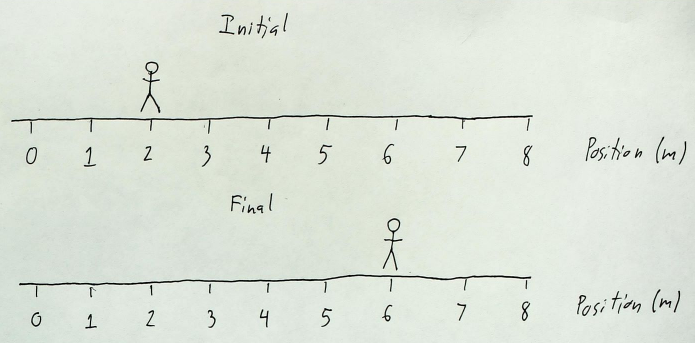
\includegraphics[scale=0.8]{example_units_velocity_walking.png}
\end{figure}

We know Alice's initial position $x_i = 2.0 \, m$ and final position $x_f = 6.0 \, m$. This means her change in position is

\begin{equation}
\Delta x = x_f - x_i
\end{equation}

\begin{equation}
\Delta x = 6.0 \, m - 2.0 \, m = 4.0 \, m
\end{equation}

In the problem we are told she walks for $8.0 \, s$, so our time duration is $\Delta t = 8.0 \, s$. Now we can use the definition of average velocity

\begin{equation}
v_{avg} = \frac{\Delta x}{\Delta t}
\end{equation}

\begin{equation}
v_{avg} = \frac{4.0 \, m}{8.0 \, s} = 0.50 \, \frac{m}{s}
\end{equation}

Her average velocity is $0.50 \, \frac{m}{s}$. Notice how we get the units of $\frac{m}{s}$ by just dividing the units in the equation.

\end{exampleblock}

The final quantity we will introduce is \textbf{speed}. This is a measurement of how fast an object is moving. You might be familiar with miles per hour (mph) or kilometers per hour ($\frac{km}{hr}$) from a car speedometer. The SI unit of speed is $\frac{m}{s}$, same as velocity. Speed will be denoted as $s$ in equations.

\textbf{Average speed} can be found by taking the distance traveled $d$ over the time duration $\Delta t$.

\begin{equation}
s_{avg} = \frac{d}{\Delta t}
\end{equation}

One important issue we must address is how average speed differs from average velocity. Both are measured in units of $\frac{m}{s}$ and can be used to get information about how fast an object moved.

\begin{enumerate}
\item Speed is a scalar quantity, not a vector quantity. Speed does not tell you anything about the direction of motion. There is no such thing as a negative speed because the distance traveled will always be zero or positive.

\item The distance traveled is not always the same as the change in position. Velocity only depends on $x_i$, $x_f$, and $\Delta t$ with no concern for the path taken between $x_i$ and $x_f$. Speed depends on the distance traveled so it does matter what the path taken is.
\end{enumerate}

The last new definitions we will introduce here are \textbf{instantaneous speed} and \textbf{instantaneous velocity}. Instantaneous speed is a measure of the speed at an instant in time. Instantaneous velocity is the rate of change in position at an instant in time, which can also be thought of as the instantaneous speed plus the direction of travel.

\section{Motion Graphs}

One helpful tool for studying the motion of objects is to use graphs. This allows us to present data in a visual format rather than text. The x-axis will be the time and the y-axis will be position, velocity, or acceleration.

First, let's start with the following graph of position vs. time (which is also called an \textit{x vs t} plot).

\begin{figure}[H]
\centering
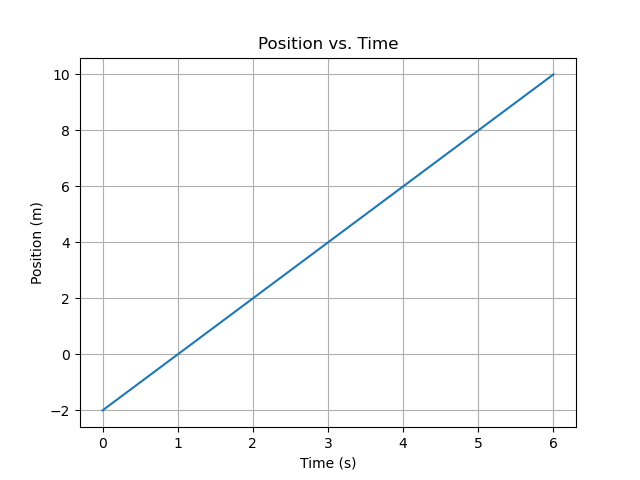
\includegraphics[scale=0.6]{position1.png}
\caption{Sample position vs. time graph}
\label{pos1}
\end{figure}

The graph has a title that tells you what the graph shows and the x- and y-axes are labeled, including units. These features are important to allow somebody reading your graph to easily understand what it is showing. 

This graph has time in seconds on the x-axis and position in meters on the y-axis. What this graph is showing is therefore the position of an object as it moves over time. For example, if we wanted to find the position of the object at $t = 4 \, s$ we would look at the y-value of the graph at $4 \, s$. The position of the object is therefore $x = 6 \, m$.

What if we wanted to find the average velocity of the object throughout this motion? It moves for 6 seconds, so $\Delta t = 6 \, s$. The position at $t = 0 \, s$ is $x = -2 \, m$, so we have in the initial state $x_i = -2 \, m$. The position at $t = 6 \, s$ is $x = 10 \, m$, so we have in the final state $x_f = 10 \, m$.

\begin{equation}
v_{avg} = \frac{\Delta x}{\Delta t} = \frac{10 \, m - (-2) \, m}{6 \, s} = 2 \, \frac{m}{s}
\end{equation}

Since our y-value is position and x-value is time, what we just did above is find the slope of the line! We can extend this in general to recognize that \textbf{the slope of a \textit{x vs t} graph is the velocity.} We can use this to find instantaneous velocities by finding the slope at a point on the graph! Below is a plot of velocity vs. time that describes the same motion.

\begin{figure}[H]
\centering
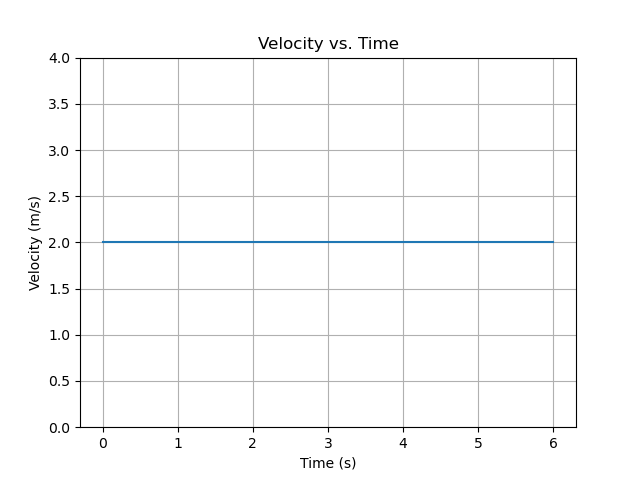
\includegraphics[scale=0.6]{velocity1.png}
\caption{Sample velocity vs. time graph for the same motion as \ref{pos1}.}
\end{figure}

The slope of the \textit{x vs t} plot is constant, so the velocity doesn't change throughout the motion. From $0 \, s$ to $6 \, s$ we have $v = 2 \, \frac{m}{s}$. Next lets look at what we call the ``area under the curve'', which is the area of the graph between the x-axis and the graph value. Since the velocity is constant, the area is just a rectangle

\begin{equation}
Area = 2.0 \, \frac{m}{s} \cdot 6 \, s = 12 \, m
\end{equation}

Back to the \textit{x vs t} plot where we had $x_f = 10 \, m$ and $x_i = -2 \, m$, we have a change in position

\begin{equation}
\Delta x = x_f - x_i = 10 \, m - (-2) \, m = 12 \, m
\end{equation}

\textbf{The area under the graph of a \textit{v vs t} graph is the change in position of the object!} Since the y-axis is velocity and the x-axis is time, we are multiplying the velocity by the time to get the change in position. Note that the \textit{v vs t} graph does not tell us what the value of $x_i$ is, just how much the position changes by.


This is a good time to make a very important point: \textbf{motion graphs are not a ``picture'' of the motion, but instead a visual representation of data}. The \textit{x vs t} and \textit{v vs t} look very different from each other despite describing the same motion. That is because they show how the position and velocity change over time, not provide a ``picture'' of how the object moves. In almost every case the position, velocity, and acceleration graphs for a moving object will all look very different from each other.

Using the same rational as above, the acceleration is the slope of the \textit{v vs t} graph and the change in velocity is the area under the \textit{a vs t} graph. We will try these concepts out in the example below.

\begin{exampleblock}

The acceleration of an object over time is measured as

\begin{table}[h]
\large
\centering
\caption{Acceleration vs Time example}
\begin{tabular}{| c | c |}
	\hline
	Time ($s$) & Acceleration ($m/s^2$) \\
	\hline
	0 & 9 \\ \hline
	1 & 7 \\ \hline
	2 & 5 \\ \hline
	3 & 3 \\ \hline
	4 & 1 \\ 
	\hline
\end{tabular}
\label{atable_ex1}
\end{table}

\begin{enumerate}
\item Plot the acceleration vs. time.
\item Use the acceleration vs. time graph to create a velocity vs. time graph if the velocity at $t = 0 \, s$ is $v = -4 \, m/s$.
\end{enumerate}

First we can create our \textit{a vs. t} plot with time on the x-axis and acceleration on the y-axis. We can see the plot in \ref{atable_motiongraph_ex1}, where the data points have been plotted and fit with a line.

\begin{figure}[h]
\centering
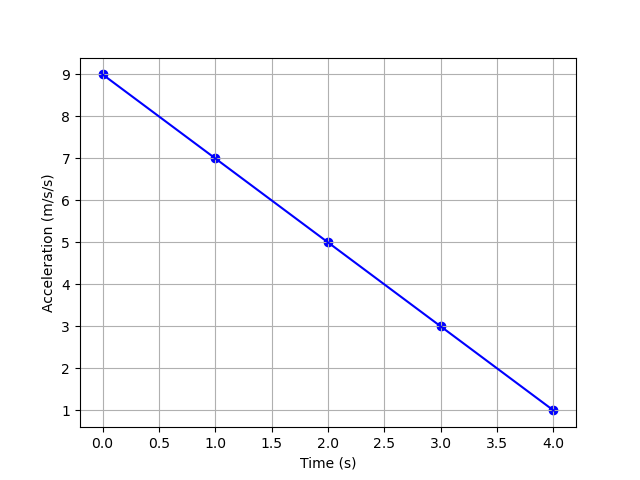
\includegraphics[scale=0.6]{example_accel.png}
\caption{Graph created from data in \ref{atable_ex1}}
\label{atable_motiongraph_ex1}
\end{figure}

We see that the acceleration changes linearly (as a straight line) with time. The acceleration is positive and decreasing over the entire duration of the graph.

Now we can use the \textit{a vs. t} graph to create our \textit{v vs. t} graph. The change in velocity over time is the area under the curve of the \textit{a vs. t} graph. With the acceleration changing over time, how can we find the area under the curve?

Let's focus first on the interval $t = 0 \, s$ to $t = 1 \, s$. The acceleration is linear, so the average acceleration over the interval is 

\begin{equation}
a_{avg} = \frac{a(t=0) + a(t=1)}{2}
\end{equation}

The acceleration is a function of time, so $a(t=0)$ means the acceleration at $t = 0 \, s$ and $a(t=1)$ means the acceleration at $t = 1 \, s$. The average acceleration between $t = 0 \, s$ and $t = 1 \, s$ is

\begin{equation}
a_{avg} = \frac{9 \, m/s^2 + 7 \, m/s^2}{2} = 8 \, \frac{m}{s^2}
\end{equation}

The area under the curve is the average acceleration multiplied by the time, which is $1 \, s$ for this interval

\begin{equation}
\Delta v = a_{avg} \cdot \Delta t
\end{equation}

\begin{equation}
\Delta v = (8 \, \frac{m}{s^2}) (1 \, s) = 8 \, \frac{m}{s}
\end{equation}

The velocity at $t = 1 \, s$ is the velocity at $t = 0 \, s$ plus the change in velocity between $t = 0 \, s$ and $t = 1 \, s$.

\begin{equation}
v(t=1) = v(t=0) + \Delta v
\end{equation}

\begin{equation}
v(t=1) = -4 \, \frac{m}{s} + 8 \, \frac{m}{s} = 4 \, \frac{m}{s}
\end{equation}

Try repeating this process for each one second interval. The velocities that you should get are shown in \ref{vtable_ex1}.

\begin{table}[h]
\large
\centering
\caption{Velocity vs Time example}
\begin{tabular}{| c | c |}
	\hline
	Time ($s$) & Velocity ($m/s$) \\
	\hline
	0 & -4 \\ \hline
	1 & 4 \\ \hline
	2 & 10 \\ \hline
	3 & 14 \\ \hline
	4 & 16 \\ 
	\hline
\end{tabular}
\label{vtable_ex1}
\end{table}



\begin{figure}[h]
\centering
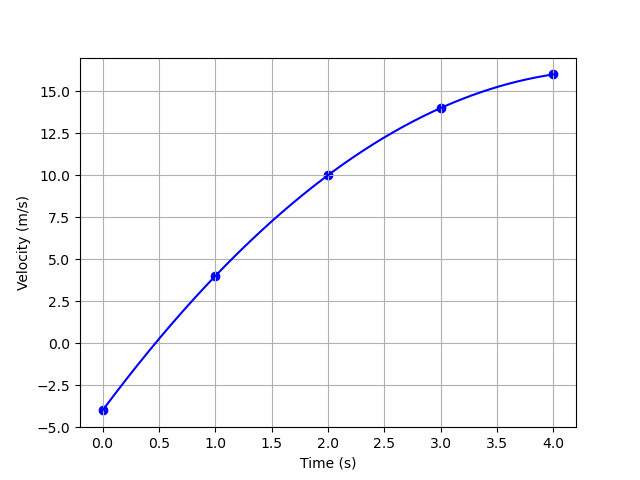
\includegraphics[scale=0.6]{example_vel.png}
\caption{Velocity vs time graph created from the data in \ref{atable_ex1} and initial condition of $v = -4 \frac{m}{s}$ at $t = 0 \, s$.}
\end{figure}

This graph is a parabola which opens downward. If you are taking or have taken calculus, you would recognize this as being the integral of the \textit{a vs. t} graph. 

\end{exampleblock}

\newpage

\section{Constant Acceleration Motion}

One case of particular interest we will look at is \textbf{constant acceleration motion}, where the acceleration does not change over an interval of time. This is useful for 2 reasons:

\begin{enumerate}
\item Common. There are several examples of constant acceleration motion or motion that is close enough to having a constant acceleration that we can approximate it as such. This gives us a useful way to describe a variety of physical situations.

\item Easy to work with mathematically.
\end{enumerate}

We will start by saying that acceleration is constant as a function of time

\begin{equation}
\begin{split}
a(t) = a \\
a_i = a_f = a
\end{split}
\end{equation}

Now we will consider motion from a time of zero ($t = 0 \, s$) to some later time $t$. This means that our $\Delta t$ is

\begin{equation}
\Delta t = t - 0 = t
\end{equation}

Now we can work with our definition of average acceleration. If the acceleration is constant, then the average acceleration is the constant value of acceleration $a_{avg} = a$. Let's see if we can find the velocity $v_f$ at a time $t$ starting with the definition of acceleration.

\begin{equation}
a = \frac{\Delta v}{\Delta t}
\end{equation}

\begin{equation}
a = \frac{v_f - v_0}{t}
\end{equation}

Above we see a subscript zero for the first time. The variable $v_0$ is pronounced ``v naught'' and is used to indicated the value of a motion variable at time zero. It is the special case of the initial state being at time zero.

Continuing on with the equation, we can multiply both sides by $t$.

\begin{equation}
at = v_f - v_0
\end{equation}

Now we can add $v_0$ to both sides to get.

\begin{equation}
v_f = v_0 + at
\label{km1}
\end{equation}

Which gives us the final velocity $v_f$ at a time $t$ given the velocity at $t = 0 \, s$ is $v_0$ and the acceleration is a constant value of $a$. This is the first of the \textbf{kinematic equations}, which are used to describe constant acceleration motion.

Constant acceleration motion has a linear velocity, which means we can find the average velocity as 

\begin{equation}
v_{avg} = \frac{v_0 + v_f}{2}
\label{kmvavg1}
\end{equation}

From the definition of average velocity, we also have 

\begin{equation}
v_{avg} = \frac{\Delta x}{t}
\label{kmvavg2}
\end{equation}


Now we can set the right hand sides of \ref{kmvavg1} and \ref{kmvavg2} equal and solve for $\Delta x$

\begin{equation}
\frac{\Delta x}{t} = \frac{v_0 + v_f}{2}
\end{equation}

\begin{equation}
\Delta x = \frac{v_0 + v_f}{2} \cdot t
\label{km2}
\end{equation}

This is the second kinematic equation, used for finding the change in position if we know the initial and final velocities. We can get a third kinematic equation that does not include $v_f$ if we use the definition of $v_f$ from equation \ref{km1} and plug that into equation \ref{km2}.

\begin{equation}
\Delta x = \frac{v_0 + v_0 + at}{2} \cdot t
\end{equation}

\begin{equation}
x_f - x_0 =  (v_0 + \frac{1}{2}at) \cdot t
\end{equation}

\begin{equation}
x_f = x_0 + v_0 t + \frac{1}{2} a t^2
\label{km3}
\end{equation}

This is the third kinematic equation and gives us the final position as a function of initial quantities.

So far, these 3 kinematic equations have all included time as a variable. What if we don't know or care about the time but want to study how other quantities are related. Let's return to \ref{km1} and solve for time $t$.

\begin{equation}
v_f = v_0 + at
\end{equation}

\begin{equation}
v_f - v_0 = at
\end{equation}

\begin{equation}
t = \frac{v_f - v_0}{a}
\end{equation}

Now we can take this expression for $t$ and plug it into \ref{km3}.

\begin{equation}
x_f = x_0 + v_0 \left( \frac{v_f - v_0}{a} \right) + \frac{1}{2} a \left( \frac{v_f - v_0}{a} \right)^2
\end{equation}

We can simplify by moving $x_0$ and working with the terms in parentheses.

\begin{equation}
x_f - x_0 = \frac{1}{a} (v_f v_0 - v_0^2) + \frac{1}{2}a \left( \frac{v_f^2 - 2 v_f v_0 + v_0^2}{a^2} \right)
\end{equation}

This may look like a mess but don't worry, we will get a nice equation when we are done. We will replace $x_f - x_0$ with $\Delta x$, since that is the definition of the change in position. Also, we will simplify the second term on the right hand side by distributing the $\frac{1}{2}$ and pulling $\frac{1}{a^2}$ out of the parentheses.

\begin{equation}
\Delta x = \frac{1}{a} (v_f v_0 - v_0^2) + \frac{1}{a} (\frac{1}{2} v_f^2 - v_f v_0 + \frac{1}{2} v_0^2)
\end{equation}

If we multiply both sides by $a$, we can remove the parentheses and group the like terms on the right hand side.

\begin{equation}
a \Delta x = v_f v_0 - v_0^2 + \frac{1}{2} v_f^2 - v_f v_0 + \frac{1}{2} v_0^2
\end{equation}

\begin{equation}
a \Delta x = \frac{1}{2} v_f^2 + v_f v_0 - v_f v_0 + \frac{1}{2} v_0^2 - v_0^2
\end{equation}

The $v_f v_0$ cross terms actually cancel out!

\begin{equation}
a \Delta x = \frac{1}{2} v_f^2 - \frac{1}{2} v_0^2
\end{equation}

Now we can solve this equation for $v_f^2$.

\begin{equation}
2 a \Delta x	 = v_f^2 - v_0^2
\end{equation}

\begin{equation}
v_f^2 = v_0^2 + 2 a \Delta x
\label{km4}
\end{equation}

Here we have the fourth kinematic equation, which does not include time but instead the change in position, initial velocity, final velocity, and acceleration.

All of the equations are collected in \ref{kmtable}. When presented with a problem, looking at what variable each kinematic equation is missing can help you choose what equation to use. We will go through a few examples and walk through problem solving in more detail. Throughout studying motion with kinematic equations, you need to remember that \textbf{we can only use the kinematic equations with constant acceleration motion}. We derived these equations from the starting point of constant acceleration, so if acceleration changes then these equations are no longer valid. 

\begin{table}[b]
\large
\centering
\caption{Kinematic Equations}
\label{kmtable}
\begin{tabular}{| c | c | c |}
	\hline
	Equation number & Formula & Missing variable \\
	\hline
	1 & $v_f = v_0 + at$ & No position \\[5pt] \hline
	2 & $\Delta x = \frac{v_0 + v_f}{2} \cdot t$ & No acceleration \\[5pt] \hline
	3 & $x_f = x_0 + v_0 t + \frac{1}{2} a t^2$ & No final velocity \\[5pt] \hline
	4 & $v_f^2 = v_0^2 + 2 a \Delta x$ & No time \\[5pt]
	\hline
\end{tabular}
\end{table}

\newpage


\section{Problem Solving with Kinematic Equations}

We can follow a basic outline to solving constant acceleration problems using kinematic equations. A typical problem will have a couple sentences describing a physical scenario and asking for a quantity of the motion. When approaching a problem, you should go use the following steps:

\begin{enumerate}
\item Identify the known quantities in the problem. This is the information the problem gives you. Drawing a picture is often useful!

\item Identify the quantity that we are trying to solve for.

\item Choose a kinematic equation that contains the known quantities and the one we wish to solve for.

\item Solve the kinematic equation algebraically for the quantity of motion we are trying to find. Do not plug in numbers before doing this!

\item Plug in numbers and solve the problem.
\end{enumerate}

It is important to not plug in numbers early because that makes it difficult to find any mistakes in the solution. Finding algebra mistakes with variables is much easier than finding mistakes with numbers.

\begin{exampleblock}

A ball rolling down a ramp accelerates at $3.0 \, m/s^2$. If the ramp is $L = 2.5 \, m$ long and the ball is released from rest at the top of the ramp, how what is the velocity of the ball when it reaches the bottom of the ramp?

\begin{figure}[h]
\centering
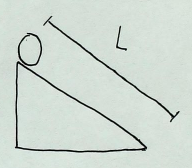
\includegraphics[scale=0.8]{example_units_ball_ramp.png}
\end{figure}

\hspace{10pt}

First we can take stock of what we know. We have the acceleration $a = 3.0 \, m/s^2$ given. The ball travels from the top to the bottom of the ramp, so the change in position is the length of the ramp $\Delta x = 2.5 \, m$. That may look like all of the given information, but there is one more thing we are given. The problem states that the ball ``is released from rest'', which means that the ball is stationary when the motion starts (``at rest'' means it is still or stationary). Therefore, we also know that $v_0 = 0 \, m/s$.

We want to solve for the velocity at the bottom of the ramp. This is the final state of the problem, so that is our final velocity $v_f$.

We don't have time, so it makes sense to look at the 4th kinematic equation.

\begin{equation}
v_f^2 = v_0^2 + 2 a \Delta x
\end{equation}

The only value we don't have here is $v_f$, so this will work. Let's take the square root of both sides to solve for velocity.

\begin{equation}
v_f = \sqrt{v_0^2 + 2 a \Delta x}
\end{equation}

Plug in numbers.

\begin{equation}
v_f = \sqrt{(0 \, m/s)^2 + 2 (3.0 \, m/s^2) (2.5 \, m)}
\end{equation}

\begin{equation}
v_f = \sqrt{15 \, m^2 / s^2} = 3.9 \, m/s
\end{equation}

The ball has a velocity of $3.9 \, m/s$ when it reaches the bottom of the ramp. Notice how tracking the units shows we get units of $m/s$ at the end to help us verify that our work was correct. This is why it is good to track units!

\end{exampleblock}

\begin{exampleblock}

A car that is driving at $34.0 \, m/s$ begins to brake, slowing down at $1.50 \, m/s^2$. If the car ends at a velocity of $28.0 \, m/s$, how much time was it slowing down for?

\hspace{10pt}

We know that the car starts at a velocity of $v_0 = 34.0 \, m/s$ and ends at a velocity of $v_f = 28.0 \, m/s$. The acceleration of the car is causing it to slow down, which means the acceleration is in the opposite direction as the velocity. Therefore, the acceleration is negative, with a value of $a = -1.50 \, m/s^2$.

We need to solve for the time $t$ that it takes to change from $v_0$ to $v_f$ with an acceleration $a$. This means we want to use the 1st kinematic equation.

\begin{equation}
v_f = v_0 + at
\end{equation}

Now we can solve this algebraically for $t$.

\begin{equation}
v_f - v_0 = at
\end{equation}

\begin{equation}
t = \frac{v_f - v_0}{a}
\end{equation}

Now we can plug in numbers

\begin{equation}
t = \frac{28.0 \, m/s - 34.0 \, m/s}{-1.50 \, m/s^2} = \frac{-6.0 \, m/s}{-1.50 \, m/s^2} = 4.00 \, s
\end{equation}

The car has to hit the brakes for $4.00 \, s$ to slow down as described in the problem. 

\end{exampleblock}

The general outline to problem solving here will be useful throughout your studies in physics. The variables and equations involved will change, but the method remains the same.

\section{Significant Digits and Uncertainty}
Now that we are able to solve motion problems with kinematic equations we need to discuss \textbf{significant digits}. As the name implies, these are the digits that are significant in the answer. They specifically give us information about the \textbf{precision} of a given value. What we mean by precision is how large a range we know a given value lies in. In the real world we cannot measure anything perfectly, there will always be \textbf{uncertainty} in the measured number. The number of significant digits tells us about the uncertainty in a number.

As an example, let's compare the times $4.0 \, s$ and $4.00 \, s$. In mathematics, these numbers are no different. In physics, the extra zero in $4.00 \, s$ tells us that we have a more precise knowledge of the value than $4.0 \, s$ would imply. As a rule of thumb, there is uncertainty in the last reported digit. That is the wiggle room in which the actual value could lie. In this example, we could know the actual value of $4.00 \, s$ is somewhere between $3.99 \, s$ and $4.01 \, s$, while the actual value of $4.0 \, s$ is somewhere between $3.9 \, s$ and $4.1 \, s$. This is how the extra zero implies our answer has greater precision.

Throughout this text, we will typically use 2 or 3 significant digits. You should give an answer in the same number of significant digits as the values given in the problem so that you report an answer to the same precision as the values you used to do the calculation.

When you take measurements of your own, you should report a value with an uncertainty to represent the range in which the actual value could lie. We typically do this by reporting in the form 

\begin{equation}
value \pm uncertainty
\end{equation}

where the ``plus-minus'' tells us the range is from $value - uncertainty$ to $value + uncertainty$. When doing operations with measured values, use the correct number of significant digits for your measured quantities and report your results in the correct number of significant digits.

For finding the uncertainty in your measured value, it makes sense to look at an example with division. Suppose we measure a change in position and a time with some uncertainty.

\begin{equation}
\Delta x = x_1 \pm \delta x_1
\end{equation}

\begin{equation}
\Delta t = t_1 \pm \delta t_1
\end{equation}

The velocity will have an uncertainty based on the uncertainties in the position and velocity. We would find that uncertainty with

\begin{equation}
\delta v_1 = \sqrt{(\delta x_1)^2 + (\delta t_1)^2}
\end{equation}

To give us 

\begin{equation}
v = v_1 \pm \delta v_1
\end{equation}

This works for multiplication and division. What about addition and subtraction? For this we can simply add the uncertainties. For example, let's suppose we measure 

\begin{equation}
x_i = x_1 \pm \delta x_1
\end{equation} 

\begin{equation}
x_f = x_2 \pm \delta x_2
\end{equation}

Say we want to find the change in position $\Delta x = x_3 = x_2 - x_1$. The uncertainty is

\begin{equation}
\delta x_3 = \delta x_1 + \delta x_2
\end{equation}

\begin{equation}
\Delta x = x_3 \pm \delta x_3
\end{equation}

For addition and subtraction we just add the uncertainties.

\section{Gravity and Free-fall}
\label{gravsec}

One common scenario where we have constant acceleration is when an object is being acted on by gravity at the Earth's surface. At the Earth's surface, \textbf{gravity} causes an object to accelerate straight down toward to the center of the Earth. When an object is accelerating only due to gravity, we call that \textbf{free-fall}. Free-fall ignores other effects like air resistance (which we will talk about more later), so it works in cases where those effects are very small. An example is a thrown baseball. While the ball is airborne, the only acceleration it experiences is gravity. 

Since free-fall is a special case that we will regularly encounter, we use the variable $g$ to denote free-fall acceleration. The acceleration due to gravity is 

\begin{equation}
g = 9.8 \, \frac{m}{s^2}
\end{equation}

directed straight down. If we define up as positive, then $a = -g$. If we define down as positive, then $a = g$.

\begin{exampleblock}

Mary drops a rock from a bridge that is $6.0 \, m$ above the water. If she releases the rock from rest, how much time does it take for the rock to hit the water?

\hspace{10pt}

First we need to define our position coordinates to determine if up or down is positive. Let's say that the water is at a height of $0 \, m$ and the bridge is at a height of $6.0 \, m$. This means that $x_0 = 6.0 \, m$ and $x_f = 0.0 \, m$. Since up is positive, we know that the acceleration is $a = -g = -9.8 \, \frac{m}{s^2}$. Mary releases the rock from rest, so $v_0 = 0 \, m/s$.

We are trying to solve for the time $t$. Based on what we have, it makes the most sense to use the 3rd kinematic equation.

\begin{equation}
x_f = x_0 + v_0 t + \frac{1}{2} a t^2
\end{equation}

This is a quadratic equation for time, and we are trying to solve for time. In general we would have to use the quadratic formula. However, if we plug in $v_0 = 0 \, m/s$, the term that is linear in $t$ (has $t$ to the first power) cancels out and we can solve it more easily.

\begin{equation}
x_f = x_0 + \frac{1}{2} a t^2
\end{equation}

\begin{equation}
\frac{1}{2} a t^2 = x_f - x_0
\end{equation}

\begin{equation}
t^2 = \frac{2}{a} (x_f - x_0)
\end{equation}

\begin{equation}
t = \sqrt{\frac{2}{a} (x_f - x_0)}
\end{equation}

\begin{equation}
t = \sqrt{\frac{2}{-9.8 \, m/s^2} (0 \, m - 6.0 \, m)}
\end{equation}

\begin{equation}
t = \sqrt{\frac{2}{-9.8 \, m/s^2} (-6.0 \, m)}
\end{equation}

The negative signs cancel, so we have a positive value in the radical.

\begin{equation}
t = \sqrt{\frac{2 \cdot 6.0 \, m}{9.8 \, m/s^2}} = 1.2 \, s
\end{equation}

The rock will hit the water $1.2 \, s$ after she drops it.

\end{exampleblock}

One thing to remember is that an object that is airborne will always be accelerated at a magnitude $g$ straight down. Magnitude here means the number, so the acceleration is always $9.8 \, \frac{m}{s^2}$ downward. This is true whether an object is rising or falling. The acceleration is not necessarily in the same direction as the velocity!

One question that we will often look at is the maximum height an object reaches when it is thrown or launched upward. When studying this the final state is when the object reaches its maximum height. \textbf{If an object is initially moving straight upward, at the highest point its velocity is zero.} We can think about this by thinking about how the velocity changes. On the way up, the velocity is upward. As it falls back down, the velocity is downward. The highest point is where the velocity crosses zero when switching form upward to downward.

\begin{exampleblock}

Rocky tosses a ball straight up in the air at a velocity of $12.0 \, m/s$. He releases the ball at a height of $h = 1.8 \, m$ off the ground. What is the maximum height the ball reaches?

\hspace{10pt}

We will call up positive so that the initial velocity is $v_0 = 12.0 \, m/s$. The initial position is the starting height, so $x_0 = 1.8 \, m$. The final state is the highest point the ball reaches, so its final velocity is zero $v_f = 0 \, m/s$. The ball is in free-fall and up is positive, so $a = -g = -9.8 \, \frac{m}{s^2}$.

Finding the highest point means we want the position in the final state, so we are solving for $x_f$. Looking at the kinematic equations none of them look quite right at first glance, but remember the definition of change in position is $\Delta x = x_f - x_0$. With that, we can use the 4th kinematic equation.

\begin{equation}
v_f^2 = v_0^2 + 2 a \Delta x
\end{equation}

\begin{equation}
v_f^2 = v_0^2 + 2 a (x_f - x_0)
\end{equation}

Now we can solve for $x_f$.

\begin{equation}
v_f^2 - v_0^2 = 2 a (x_f - x_0)
\end{equation}

\begin{equation}
\frac{v_f^2 - v_0^2}{2 a} = x_f - x_0
\end{equation}

\begin{equation}
x_f = \frac{v_f^2 - v_0^2}{2 a} + x_0
\end{equation}

\begin{equation}
x_f = \frac{(0 \, m/s)^2 - (12.0 \, m/s)^2}{2 \cdot (-9.8 \, m/s^2)} + 1.8 \, m
\end{equation}

\begin{equation}
x_f = \frac{144 \, (m/s)^2}{19.6 \, m/s^2} + 1.8 \, m = 9.1 \, m
\end{equation}

The ball reaches a maximum height of $9.1 \, m$ off the ground.

\end{exampleblock}

\section{Motion in 2 Dimensions}
\label{2Dmotion}

So far we have only talked about motion in one dimension, such as an object falling straight down or sliding along the floor. So how do we handle objects that don't move along along a straight line? This is called \textbf{2 dimensional (2D) motion}. We can split the motion along 2 perpendicular axes and treat those separately! This will often be a horizontal and vertical split, but can be any perpendicular directions. The standard convention is that horizontal motion is denoted with an $x$ and vertical motion is denoted with a $y$.

\begin{table}[b]
\large
\centering
\caption{Kinematic Equations in 2 Dimensions}
\label{kmtable}
\begin{tabular}{| c | c | c |}
	\hline
	Equation number & $x$ & $y$ \\
	\hline
	1 & $v_{f,x} = v_{0,x} + a_x t$ & $v_{f,y} = v_{0,y} + a_y t$ \\[5pt] \hline
	2 & $\Delta x = \frac{v_{0,x} + v_{f,x}}{2} \cdot t$ & $\Delta y = \frac{v_{0,y} + v_{f,y}}{2} \cdot t$ \\[5pt] \hline
	3 & $x_f = x_0 + v_{0,x} t + \frac{1}{2} a_x t^2$ & $y_f = y_0 + v_{0,y} t + \frac{1}{2} a_y t^2$ \\[5pt] \hline
	4 & $v_{f,x}^2 = v_{0,x}^2 + 2 a_x \Delta x$ & $v_{f,y}^2 = v_{0,y}^2 + 2 a_y \Delta y$ \\[5pt]
	\hline
\end{tabular}
\end{table}

We use the subscript $x$ and $y$ to denote which axis we are looking at. Notice how all positions, velocities (initial and final), and accelerations are split along the axes. The only connection between the 2 axes is the time! For example, we can find the time when an object hits the ground using the y-axis motion and use that time to find how far along the x-axis it moved.

\begin{exampleblock}

Chris throws a rock horizontally off a bridge at $4.5 \, \frac{m}{s}$. If the surface of the water is $12 \, m$ below where they threw the rock from, how far (horizontally) from the bridge does the rock hit the water?

\hspace{10pt}

Let's take stock of what we know along the $x$ and $y$ directions. We know that Chris throws the rock horizontally, so the entire velocity is along the $x$ direction. Define up as positive $y$, and the direction they throw the rock as positive $x$.

\begin{itemize}
\item $v_{0,x} = 4.5 \, \frac{m}{s}$
\item $v_{0,y} = 0 \, \frac{m}{s}$
\item $a_y = -g = -9.8 \, \frac{m}{s^2}$
\item $a_x = 0 \, \frac{m}{s^2}$
\item $y_0 = 12.0 \, m$
\item $y_f = 0 \, m$
\end{itemize}

We can also set $x_0 = 0 \, m$ and we will want to find $x_f$. The first thing that we need to do is use the vertical motion to determine how long the rock takes to fall.

\begin{equation}
y_f = y_0 + v_{0,y} t + \frac{1}{2} a_y t^2
\end{equation}

Plug in $v_{0,y} = 0 \, \frac{m}{s}$ and $y_f = 0 \, m$ to simplify the algebra.

\begin{equation}
-y_0 = \frac{1}{2} a_y t^2 
\end{equation}

\begin{equation}
t = \sqrt{\frac{-2 y_0}{a_y}}
\end{equation}

\begin{equation}
t = \sqrt{\frac{-2 (12.0 \, m}{(-9.8 \, m/s^2)}} = 1.56 \, s
\end{equation}

Now we can use this time to solve for $x_f$

\begin{equation}
x_f = x_0 + v_{0,x} t + \frac{1}{2} a_x t^2
\end{equation}

Since $x_0 = 0 \, m$ and $a_x = 0 \, \frac{m}{s^2}$, when we plug in numbers we get:

\begin{equation}
x_f = (4.5 \, \frac{m}{s}) (1.56 \, s) = 7.0 \, m
\end{equation}

The rock will hit the water at a horizontal distance of $7.0 \, m$ from where Chris threw it.

\end{exampleblock}

%We can also represent the 2D motion with vectors. For example, a 2D acceleration would be written as 

%\begin{equation}
%a = (a_x \, \hat{i}, a_y \, \hat{j})
%\end{equation}

%The $\hat{i}$ and $\hat{j}$ are \textbf{unit vectors} that indicate direction. By convention $\hat{i}$ is in the x-direction, $\hat{j}$ is in the y-direction, and $\hat{k}$ is in the z-direction. We can use kinematic equations separately on the components to analyze the motion of an object.

%\begin{exampleblock}

%An object has initial position $x_0 = (2.0 \, \hat{i}, -3.0 \, \hat{j})$

%\end{exampleblock}

To split the motion of an object along 2 axes we will use trigonometry. See how the vector and components form a right triangle in Figure \ref{velangle}. The opposite side of the triangle is $v_y$ and the adjacent side of the triangle is $v_x$. This means we can relate the components to the original velocity as:

\begin{equation}
v_x = v \, cos(\theta)
\end{equation}

\begin{equation}
v_y = v \, sin(\theta)
\end{equation}

\begin{figure}[t]
\centering
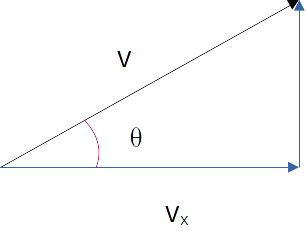
\includegraphics[scale=0.4]{Velocity_Angle.png}
\caption{Shows the vector representation of $v_x$ and $v_y$ for a velocity vector $v$ at an angle $\theta$ above the $x$-axis. Notice how this is a right triangle with the components as the legs and the velocity as the hypotenuse.}
\label{velangle}
\end{figure}

\begin{exampleblock}

A potato cannon is a device that uses compressed air to launch a potato out of a tube at a high speed. If such a potato cannon is aimed at an angle of $30.0^{\circ}$ above the ground and a potato is fired with an initial velocity of $38.0 \, \frac{m}{s}$, what are the horizontal and vertical components of the initial velocity?

\hspace{10pt}

We are given that $v_0 = 38.0 \, \frac{m}{s}$ and $\theta = 30.0^{\circ}$. Since the angle is above horizontal, the horizontal component is the adjacent side of the right triangle and the vertical component is the opposite side of the right triangle. First the horizontal component

\begin{equation}
v_{0,x} = v_0 \, cos(\theta) = (38.0 \, \frac{m}{s}) \, cos(30^{\circ}) = 29.9 \, \frac{m}{s}
\end{equation}

Now the horizontal component

\begin{equation}
v_{0,y} = v_0 \, sin(\theta) = (38.0 \, \frac{m}{s}) \, sin(30^{\circ}) = 23.4 \, \frac{m}{s}
\end{equation}

The horizontal component of the velocity is $v_{0,x} = 29.9 \frac{m}{s}$ and the vertical component of the velocity is $v_{0,y} = 23.4 \, \frac{m}{s}$.

\end{exampleblock}

\section{Projectile Motion}

One specific example of 2D motion that we will explore further is \textbf{projectile motion}, which is motion where the only acceleration is the free-fall acceleration of gravity. We ignore effects of air resistance so it is an \textit{approximation} of the physical world. This approximation is good for small objects moving at slower speeds. The assumption of free-fall acceleration tells us what the acceleration is (we will treat up as positive for this entire section)

\begin{equation}
a_y = -g = -9.8 \, \frac{m}{s^2}
\end{equation}

\begin{equation}
a_x = 0 \, \frac{m}{s^2}
\end{equation}

We will return back to the potato cannon from the end of the previous section for our study of projectile motion. The potato cannon fires a potato at initial velocity $v_0$ at an angle of $\theta$ above horizontal. This gives us

\begin{equation}
v_{0,x} = v_0 \, cos(\theta)
\end{equation}

\begin{equation}
v_{0,y} = v_0 \, sin(\theta)
\end{equation}

Let's suppose that the potato cannon is fired over level ground and we want to know how far from the cannon the potato will land. Level ground here means that the potato will land at the same height it was launched from. We are trying to solve for $\Delta x$ under the condition that $\Delta y = 0 \, m$. First we can use the vertical equation to find the time that the potato is airborne

\begin{equation}
y_f = y_0 + v_{0,y} t + \frac{1}{2} a_y t^2
\end{equation}

\begin{equation}
y_f - y_0 = (v_{0,y} + \frac{1}{2} a_y t) \cdot t
\end{equation}

Since we are on the condition that $\Delta y = 0 \, m$ we know that that $y_f - y_0 = 0 \, m$.

\begin{equation}
0 = (v_{0,y} + \frac{1}{2} a_y t) \cdot t
\end{equation}

There are two solutions, one where $t = 0 \, s$ and one where $v_{0,y} + \frac{1}{2} a_y t = 0$. The $t = 0 \, s$ solution is when the potato is launched! This is not the solution of interest to us, so we will look at the nonzero solution.

\begin{equation}
0 = v_{0,y} + \frac{1}{2} a_y t
\end{equation}

\begin{equation}
\frac{-1}{2} a_y t = v_{0,y}
\end{equation}

\begin{equation}
t = \frac{2 v_{0,y}}{a_y}
\end{equation}

Now let's plug in $v_{0,y} = v_0 \, sin(\theta)$ and $a_y = -g$

\begin{equation}
t = \frac{2 v_0 \, sin(\theta)}{g}
\end{equation}

With the time, we can look at the horizontal component.

\begin{equation}
x_f = x_0 + v_{0,x} t + \frac{1}{2} a_x t^2
\end{equation}

\begin{equation}
x_f - x_0 = v_{0,x} t + \frac{1}{2} a_x t^2
\end{equation}

Remember that $\Delta x = x_f - x_0$ so we can switch the left hand side to $\Delta x$. This is where we will also replace $v_{0,x} = v_0 \, cos(\theta)$. Now we can plug in $a_x = 0 \, \frac{m}{s^2}$ from our assumption about projectile motion and $t = \frac{2 v_0 \, sin(\theta)}{g}$.

\begin{equation}
\Delta x = v_0 \, cos(\theta) \left( \frac{2 v_0 \, sin(\theta)}{g} \right)
\end{equation}

\begin{equation}
\Delta x = \frac{2 v_0^2 \, cos(\theta) \, sin(\theta)}{g}
\end{equation}

If we use the trigonometry identity

\begin{equation}
sin(2 \theta) = 2 \, cos(\theta) \, sin(\theta)
\end{equation}

We can write this as

\begin{equation}
\Delta x = \frac{v_0^2 \, sin(2 \theta)}{g}
\end{equation}

which is known as the \textbf{range equation}. This gives the horizontal distance a projectile travels before it lands at the same height it was launched from.

There is one more question of interest we should look at, and that is the maximum height a projectile reaches. The highest point is when the object switches from moving upward to downward, so it's vertical velocity is temporarily zero. We want to find $\Delta y$ for when $v_{f,y} = 0 \, m/s$. 

\begin{equation}
v_{f,y}^2 = v_{0,y}^2 + 2 a_y \Delta y
\end{equation}

Plug in our highest point condition of $v_{f,y} = 0 \, \frac{m}{s}$

\begin{equation}
0 = v_{0,y}^2 + 2 a_y \Delta y
\end{equation}

\begin{equation}
2 a_y \Delta y = - v_{0,y}^2
\end{equation}

\begin{equation}
\Delta y = \frac{-v_{0,y}^2}{2 a_y}
\end{equation}

Plug in $v_{0,y} = v_0 \, sin(\theta)$ and $a_y = -g$ to get

\begin{equation}
\Delta y = \frac{v_0^2 \, sin^2 (\theta)}{2 g}
\end{equation}

\section{Uniform Circular Motion}

While we did look a lot at constant acceleration motion throughout this chapter, there are some types of motion with varying acceleration that are simple enough for us to study. One example is \textbf{uniform circular motion}, which is defined as

\begin{itemize}
\item The object moves in a circular path.
\item The object moves at a constant speed.
\end{itemize}

This might sound like a very specific set of conditions that wouldn't be widely applicable, but it is a valuable \textit{approximation}. A major goal of physics is to find useful simplifications to difficult problems in order to study them easily. There are many physical systems in which an object moves in a way that is very close to being uniform circular motion and we can approximate them as such. This could include cars going around a curve in the road and ferris wheels.

\begin{figure}[t]
\centering
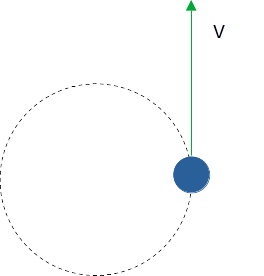
\includegraphics[scale=0.4]{UCM_vel.png}
\caption{In uniform circular motion, the instantaneous velocity is tangential (along the outside) of the circular path the object moves along.}
\label{ucm_vel}
\end{figure}

\begin{figure}[t]
\centering
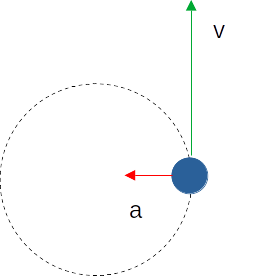
\includegraphics[scale=0.4]{UCM_accel.png}
\caption{In uniform circular motion, the instantaneous acceleration is radial, directed toward the center of the circular path the object moves along.}
\label{ucm_accel}
\end{figure}

What is the acceleration of an object in uniform circular motion? The first part of answering that is figuring out the direction of the acceleration. In order for an object to move in a circular path, its velocity must be along the circle. That means the instantaneous velocity is always \textbf{tangential} to the circle, as seen in Figure \ref{ucm_vel}. 

The speed of the object is constant so the magnitude of the velocity is constant. The direction of the velocity is always changing in order to keep the velocity tangential to the circle. As we saw in Section REF HERE, we can consider perpendicular motion separately. That means that if the force is perpendicular to the velocity, it will change the direction of the velocity without changing the magnitude of the velocity. Therefore, the acceleration is directed radially toward the center of the circle, as seen in Figure \ref{ucm_accel}. 



Now to find the magnitude of the acceleration. Doing this rigorously requires calculus but we can still get some understanding of the result.

What if the velocity increases? Increasing the velocity will increase the change in velocity. If the velocity vectors are longer, then the $\Delta v$ vector will be longer as well. Since acceleration is $a_{avg} = \frac{\Delta v}{\Delta t}$, increasing $\Delta v$ will increase the acceleration. Increasing velocity will also decrease the time interval it takes for the object to travel along the path of the circle. Decreasing $\Delta t$ will increase the acceleration.

\begin{figure}[H]
\centering
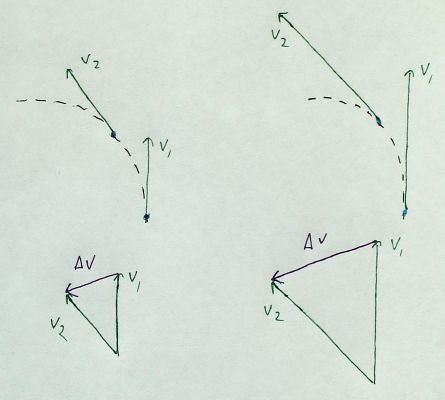
\includegraphics[scale=0.6]{ucm_dv_vel.png}
\caption{A greater velocity will result in a larger change in velocity as the object moves around the circle. That is part of the reason why increasing the velocity results in a larger acceleration.}
\end{figure}

What if the radius of the circle increases? That increases the distance the object has to move for the same change in velocity $\Delta v$. If the velocity is the same, that will increase the time required. This means that increasing the radius decreases the acceleration.

\begin{figure}
\centering
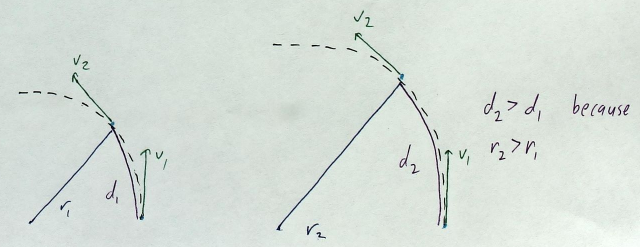
\includegraphics[scale=0.6]{ucm_dv_radius.png}
\caption{If the radius is greater, the object has to move a greater distance around the circle for the same change in velocity. This takes more time, causing the acceleration to decrease.}
\end{figure}

We have 2 ways that increasing velocity increases acceleration and 1 way that increasing radius decreases acceleration. This would lead us to propose

\begin{equation}
a_c = \frac{v^2}{r}
\label{centaccel}
\end{equation}

as the acceleration, which is in fact exactly what we would get if we did the required calculus to solve it! This acceleration is called the \textbf{centripetal acceleration}, where centripetal means directed toward the center. That's why we denote this acceleration with a subscript $c$.

The magnitude of the acceleration is constant, so why isn't this constant acceleration motion? The answer lies in the fact that the acceleration is always directed toward the center of the circle. As the object moves around the circle, the direction of the acceleration must be constantly changing so that the acceleration is always pointed toward the center of the circle. That changing direction is why the acceleration isn't constant in uniform circular motion.

\begin{exampleblock}
Alex is jogging at $2.5 \, \frac{m}{s}$ around a circular track of radius $10.0 \, m$. What is their centripetal acceleration?

We can plug in the velocity and radius into Equation \ref{centaccel}

\begin{equation}
a_c = \frac{(2.5 \, m/s)^2}{10.0 \, m} = 0.625 \, \frac{m}{s^2}
\end{equation}

Alex has a centripetal acceleration of $a_c = 0.625 \, \frac{m}{s^2}$.
\end{exampleblock}

\begin{exampleblock}
An amusement park wants a rollercoaster to have a centripetal acceleration that is ``half a g'' ($\frac{g}{2} = 4.9 \, \frac{m}{s^2}$) while going around a circular curve. If rollercoaster is moving at a velocity of $21 \, \frac{m}{s}$ around the curve, what is the radius of the curve?

First we can start with Equation \ref{centaccel} and solve for the radius.

\begin{equation}
a_c = \frac{v^2}{r}
\end{equation}

\begin{equation}
a_c r = v^2
\end{equation}

\begin{equation}
r = \frac{v^2}{a_c} = \frac{(34 \, m/s)^2}{4.9 \, m/s^2} = 90.0 \, m
\end{equation}

The radius of the curve has to be $90.0 \, m$. (You can think of this as if the curve was extended to a full circle, that circle would have a radius of 90.0 $m$.)
\end{exampleblock}

\chapter{Forces}
\setcounter{example}{1}
\addtocounter{chp}{1}

We spent the previous chapter talking about motion, but we have yet to address the physical reason \textit{why} objects move. What is the interaction that causes motion? That is the question that will motivate this chapter.

\section{Newton's Laws of Motion}

Isaac Newton (1643 - 1727) formulated 3 laws of motion that are a major foundation of physics. His laws describe how \textbf{forces} act on objects to affect their motion. Forces can be thought of as a push or pull on an object. We will go into more detail on specific forces later, but for now we can think of them as a push or pull.

\linespace

Newton's 1st Law of Motion states that:

\hspace{10pt}

\textbf{An object in motion remains in uniform motion and an object at rest remains at rest, unless acted upon by an external force}

\linespace

What this means that an object will remain in its current state unless an outside force acts on it. If the object is at rest, it will not start moving unless an outside force acts on it. If it is moving, it will keep moving at a constant velocity (meaning same speed and direction) unless a force acts on it.

\linespace

Newton's 2nd Law of Motion states that:



\hspace{10pt}

\textbf{The net force acting on an object is equal to the product of its mass and acceleration.}



\linespace

Newton's 2nd Law of Motion gives the relationship between force and acceleration. For the net force $F_{net}$, mass $m$, and acceleration $a$ we have the equation

\begin{equation}
\overrightarrow{F_{net}} = m \overrightarrow{a}
\label{2ndlaw}
\end{equation} 


Force and acceleration both being vector quantities means that the acceleration is in the same direction as the net force.

\textbf{Net force} means the sum of all forces acting on an object. In most cases objects will have 2 or more forces acting on them, so we will need to add those forces to get the net force acting on the object.

An object's mass determines its resistance to acceleration from a force. This resistance is called \textbf{inertia}. The larger the mass, the higher the inertia, and the less an object will accelerate when acted upon by a given force.

\linespace

Newton's 3rd Law of Motion states that:

\hspace{10pt}

\textbf{When object A exerts a force on object B, object B exerts a force on object A that is equal in magnitude and opposite in direction.}

\linespace

What this means is that when one object pushes on another, the second object pushes back on the first. When the law says ``equal in magnitude'', it means that the forces are the same numerical value. If object A exerts a $5 \, Newton$ force on object B, object B exerts a $5 \, Newton$ force on object A. This is also called the \textbf{action-reaction principle}. For every force, there is an equal and opposite reaction force. The reaction force has the same strength, but is in the opposite direction.

One way you can see this for yourself is to push on a wall. What happens when you do that? You will feel like you are being pushed away from the wall! That is because when you exert a force on the wall, the wall exerts an equal and opposite force on you. 



\section{Force exerted by gravity}

In Section \ref{gravsec} we looked at the acceleration due to gravity and how it is a constant acceleration $g = 9.8 \, \frac{m}{s^2}$ for any object in free-fall. Let's apply Newton's 2nd Law of Motion free-fall. Start with \ref{2ndlaw} and plug in $g$ for the acceleration.

\begin{equation}
F_{net} = mg
\end{equation}

For an object in free fall, the net force has magnitude $mg$ direction straight down. Since the only acceleration in free-fall is due to gravity, we know that the only force acting on an object in free-fall is gravity. Therefore, we can say that the force of gravity acting on an object of mass $m$ is

\begin{equation}
F_g = mg 
\label{fg}
\end{equation}

which will always be directed straight down. This force acts on any object at the Earth's surface, even if the object is not in free-fall. Early on, we said that weight is not the same as mass. \textbf{Weight} is the force of gravity acting on an object. Weight is proportional to mass, but depends on the surface gravity. This is why astronauts weighed less on the moon, despite their mass remaining constant!

\begin{exampleblock}

Lucy has to move a box that weighs 235 $N$. What is the mass of the box in kilograms?

\hspace{10pt}

Here we will use equation \ref{fg} and solve for the mass $m$.

\begin{equation}
m = \frac{F_g}{g}
\end{equation}

The force of gravity is the weight, 235 $N$.

\begin{equation}
m = \frac{235 \, N}{9.8 \, m/s^2} = 24.0 \, kg
\end{equation}

The box has a mass of $m = 24 \, kg$.

\end{exampleblock}

We can say that free-fall is when the only force acting on an object is the gravitational force

\begin{equation}
F_{net} = F_{g}
\end{equation}

\section{Normal Force}
\label{nfsec}

Set any object on the table in front of you (pencil, book, cell phone, literally anything). Is it accelerating? No! The object set on the table is sitting stationary. That means its acceleration is zero, and from Newton's first law we know that means there is no net force acting on the object.

The force of gravity is acting down on it, so there must be a force acting upward. To determine the source of the force, we can think about why the object isn't falling down. From real life experience, we can say it is obviously the table! The table stops the object from falling by exerting an upward force on the object. The force a surface exerts on an object is called the \textbf{normal force}. This is the force that keeps the object from moving ``through'' the surface. Normal force is always perpendicular to the surface, so on a perfectly horizontal table it is direction straight up. We will denote normal force as $F_N$.

\begin{exampleblock}


A book of mass $0.40 \, kg$ is sitting stationary on a table. What is the normal force acting on the book?

\hspace{10pt}

Let's call up positive. Since the book is stationary, we know its acceleration is zero and therefore the net force is zero. The gravitational force is $F_g$ directed downward. 

\begin{equation}
F_g = -mg
\end{equation}

The normal force is directed upward to make the net force zero.

\begin{equation}
F_{net} = F_N + F_g = 0 \, N
\end{equation}

\begin{equation}
F_N = -F_g = -(-mg)
\end{equation}

\begin{equation}
F_N = (0.40 \, kg) (9.8 \, \frac{m}{s^2}) = 3.9 \, N
\end{equation}

The normal force for an object sitting on a horizontal surface with no other forces acting on it is the same as the gravitational force, just directed upward.

\end{exampleblock}

\section{Forces in 2 Dimensions}
\label{2DForces}

Many physical situations have forces exerted along 2 dimensions. For example, if we have a box sitting on the floor and somebody pushes it we have 3 forces acting on the box:

\begin{enumerate}
\item Gravity acting downward.
\item Normal force acting upward.
\item The person's push acting horizontally.
\end{enumerate}

This scenario has forces that act vertically and horizontally. When studying motion like this, we can take advantage of the fact that \textbf{perpendicular forces are independent}. What this means is that a vertical force acting on an object has no impact on the horizontal motion of that object. For the box being pushed along the floor, we can analyze gravity and normal force together since they are vertical forces. Then we can look at the push separately since that is horizontal.

When we have forces that aren't perfectly horizontal or vertical, we can split them into vertical and horizontal components. Figure \ref{ForceAngle} shows how a force angled at an angle $\theta$ is split into horizontal and vertical components.

\begin{figure}[H]
\centering
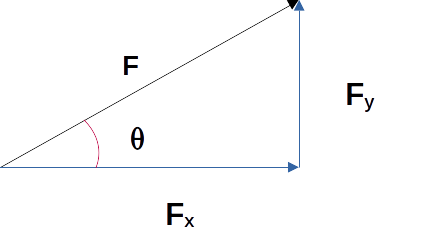
\includegraphics[scale=0.6]{Force_Angle.png}
\caption{A force directed at an angle $\theta$ above horizontal split into components. Horizontal is $F_x$ and vertical is $F_y$.}
\label{ForceAngle}
\end{figure}

You can see that the force and components form a right triangle, with the force $F$ as the hypotenuse and the components $F_x$ and $F_y$ are the legs of the right triangle. We can use \textbf{trigonometry} to find the sides. From a previous math class you should have seen the trigonometry functions sine, cosine, and tangent. They are give the relationships between the opposite leg, adjacent leg, and hypotenuse of a right triangle.

\begin{equation}
sin(\theta) = \frac{opposite}{hypotenuse}
\end{equation}

\begin{equation}
cos(\theta) = \frac{adjacent}{hypotenuse}
\end{equation}

\begin{equation}
tan(\theta) = \frac{opposite}{adjacent}
\end{equation}

From the angle $\theta$ the horizontal component is the adjacent side, so we can find $F_x$ as

\begin{equation}
F_x = F \, cos(\theta)
\end{equation}

The vertical component is the opposite side of the triangle, so we can find $F_y$ as

\begin{equation}
F_y = F \, sin(\theta)
\end{equation}

\section{Free Body Diagrams}

If we return to looking at a book on the table, we looked at a situation where there are multiple forces acting in different directions on an object. This can be difficult to keep track of as just text, so in these cases we draw pictures known as \textbf{free body diagrams}. These diagrams are simple pictures that show the forces acting on one object. The forces are drawn as arrows in the direction of the force, with the relative length of the arrows in the free body diagram showing the relative magnitudes of the forces. The free body diagram for a book sitting stationary on a table is:

FBD HERE

\section{Friction}

What happens if you slide a book across a table? It will slow down and eventually stop. From Newton's 1st Law of Motion, the change in velocity means there must be a net force. This net force is supplied by \textbf{friction}, which is the resistance to 2 surfaces sliding against each other. There are 2 types of friction:

\begin{enumerate}
\item \textbf{Kinetic friction} - acts when surfaces are sliding against each other. Slows down the moving object(s).

\item \textbf{Static friciton} - acts when the surfaces are stationary relative to each other. Acts to prevent the surfaces from moving.
\end{enumerate}

Different surfaces will have different friction forces. We know that a hockey puck will slide further on ice than on carpet before stopping, so there is a characteristic of the surfaces that determines the force. The surface interactions are described by the \textbf{coefficient of kinetic friction} and \textbf{coefficient of static friction}. In equations we will denote these coefficients with the Greek letter $\mu$, pronounced ``mu''. Subscripts are used to differentiate kinetic friction $\mu_k$ from static friction $\mu_s$. The force of kinetic friction is found by

\begin{equation}
F_k = \mu_k F_N
\label{kfriction}
\end{equation}

which is the normal force multiplied by the coefficient of kinetic friction. This means that if the coefficient of kinetic friction or the normal force increases, the force of kinetic friction increases.

\begin{exampleblock}

A box of mass $30.0 \, kg$ is sliding along a horizontal floor. The coefficient of kinetic friction between the floor and box is $\mu_k = 0.40$. What is the magnitude of kinetic friction acting on the box?

\hspace{10pt}

The normal force here can be found by looking at the vertical axis. The box is not moving up or down, so the gravitational force and normal force are equal in magnitude.

\begin{equation}
F_N = F_g = mg = (30.0 \, kg)(9.8 \, \frac{m}{s^2} = 294 \, N
\end{equation}

The force of kinetic friction is then

\begin{equation}
F_k = \mu_k F_N = 0.40 \cdot (294 \, N) = 118 \, N
\end{equation}

The force of kinetic friction on the box is $F_k = 118 \, N$

\end{exampleblock}

Notice how the coefficient of kinetic friction has no units. That is because it is multiplied by a force to find a force. It is a dimensionless (unitless) factor describing how the 2 surfaces interact when sliding along each other.

The force exerted by static friction is found by

\begin{equation}
F_s \leq \mu_s F_N
\label{sfriction}
\end{equation}

This is very similar to the force of kinetic friction, except that the coefficient is switched out for the coefficient of static friction. However, there is one major difference: \textit{the equal sign is replaced with a less than or equal sign}. That is because static friction prevents an object from starting to slide, and will not cause one surface to slide past another. In terms of Newton's Laws of Motion, static friction opposes an applied force to make the net force zero. If the applied force is larger than $\mu_s F_N$, then the static friction force is cannot make the net force zero and the object will begin sliding. 

\begin{exampleblock}

A paperweight of mass $0.75 \, kg$ is sitting on a desk. The coefficient of static friction between the desk and paperweight is $\mu_s = 0.54$. There is a force of $3.0 \, N$ pushing horizontally on the paperweight, trying to slide it on the desk. Does the paperweight slide on the desk? If not, what is the magnitude of the static friction force acting on the paperweight?

\hspace{10pt}

First we need to find out the maximum possible static friction force. First we find the normal force, which is equal to the gravitational force.

\begin{equation}
F_N = F_g = (0.75 \, kg) (9.8 \, \frac{m}{s^2}) = 7.35 \, N
\end{equation}

Now we can use Equation \ref{sfriction} to find the static friction force.

\begin{equation}
F_s \leq \mu_s F_N = 0.54 \cdot 7.35 \, N = 3.97 \, N
\end{equation}

The static friction force is less than or equal to $3.97 \, N$. This means that $3.97 \, N$ is the maximum possible static friction force. Since the applied force of $3.0 \, N$ is less than that, the static friction force can match the applied force and keep the block still.

Now to find the static friction force, we need to find the force required so that the net force is zero. 

\begin{equation}
F_{net} = F_{app} + F_s = 0
\end{equation}

If we say the applied force ($F_{app}$) is in the positive direction, we can solve the problem as such

\begin{equation}
F_s = -F_{app} = - 3.0 \, N
\end{equation}

The force of static friction is $F_s = 3.0 \, N$ in the opposite direction of the applied force. Note that $F_s$ is not always equal to $mu_s F_N$!

\end{exampleblock}





\chapter{Work, Energy, and Power}
\setcounter{example}{1}
\addtocounter{chp}{1}

Newton's Laws of Motion are a powerful tool for describing how forces cause motion, but some problems cannot be easily solved using them. In this chapter we will build off of Newton's Laws and Kinematics to develop new techniques that can be applied more broadly.

\section{Work and Kinetic Energy}

We will start with the 4th kinematic equation

\begin{equation}
v_f^2 = v_0^2 + 2 a \Delta x
\end{equation}

The right-hand side has acceleration, so we will multiply both sides by mass so that we can use Newton's 2nd Law to work with force.

\begin{equation}
m v_f^2 = m v_0^2 + 2 ma \Delta x
\end{equation}

Now we will subtract $m v_0^2$ from both sides and divide both sides by 2.

\begin{equation}
ma \Delta x = \frac{1}{2} m v_f^2 - \frac{1}{2} m v_0^2
\end{equation}

Use Newton's 2nd Law of Motion to replace $ma$ with the force $F_{net}$ to get

\begin{equation}
F_{net} \Delta x = \frac{1}{2} m v_f^2 - \frac{1}{2} m v_0^2
\label{WKEdef}
\end{equation}

The left hand side $F_{net} \Delta x$ is a quantity called \textbf{work}. Work, abbreviated $W$, is defined as a force acting over a displacement. We can find the units of work by multiplying the units of force and displacement. This gives us units of $Newtons \cdot meters$, or $N \cdot m$. This unit is called the \textbf{Joule} and is abbreviated $J$. When we treat every force acting on the object as a source of work, we call that the external work, which is abbreviated $W_{ext}$. This is an important distinction that will be important later this chapter.

The right hand side $\frac{1}{2} m v^2$ is a quantity called \textbf{kinetic energy}. Kinetic energy, abbreviated $KE$, is the energy in the motion of an object (energy is a hard quantity to define overall, so we will return to it a little later). The unit of kinetic energy is also the Joule.

This means we can write equation \ref{WKEdef} as 

\begin{equation}
W_{ext} = KE_f - KE_i = \Delta KE
\label{WKEtheorem}
\end{equation}

This is called the \textbf{work-kinetic energy theorem}, which states that the sum of all work done on an object is equal to the change in its kinetic energy. We got the initial definitions using kinematic equations, but this result applies to any forces that act over an object while it moves. This means that if we know the change in kinetic energy over some displacement, we can find the \textbf{average force} acting on that object while it was moving. The force may vary throughout, but we can find the average using work.

\begin{exampleblock}

In the previously mentioned potato cannon, the potato starts and rest and is accelerated through a tube by the compressed.

\begin{enumerate}
\item If a potato of mass $0.65 \, kg$ leaves the tube at a velocity of $32 \, \frac{m}{s}$, how much work is done on the potato?

\item If the tube is $1.6 \, m$ long, what is the force exerted on the potato?
\end{enumerate}

\hspace{10pt}

\begin{enumerate}
\item We are given $m = 0.65 \, kg$, $v_0 = 0 \, \frac{m}{s}$, and $v_f = 32 \, \frac{m}{s}$. We can use the work-kinetic energy theorem to find the work done on the potato.

\begin{equation}
W_{ext} = \frac{1}{2} (0.65 \, kg) (32 \, \frac{m}{s})^2 - \frac{1}{2} (0.65 \, kg) (0 \, \frac{m}{s})^2 = 312 \, J
\end{equation}

The cannon does $W = 312 \, J$ of work on the potato.

\item Knowing the length of the tube tells us that $\Delta x = 1.6 \, m$. We can use the definition of work $W = F \Delta x$ to find the average force.

\begin{equation}
W = F \Delta x
\end{equation}

\begin{equation}
F = \frac{W}{\Delta x} = \frac{312 \, J}{1.6 \, m} = 195 \, N
\end{equation}

The average force acting on the potato in the tube is $F = 195 \, J$. 

\end{enumerate}

\end{exampleblock}

\section{Direction of Force}

In the previous section we only talked about accelerations and forces in 1 dimension, where they are aligned with the displacement. But what about forces that aren't along the same axis as the displacement? In Section \ref{2DForces} we saw that forces can be split into perpendicular components, where the two components are completely independent. This result tells us that \textbf{work is only done by components of the force in the same axis of the motion}. Forces (or the components of forces) perpendicular to the motion do no work!



Suppose we have a force $F$ and displacement $\Delta x$ that are separated by an angle $\theta$ as shown in Figure \ref{work_angle}. The component of force along the displacement is the adjacent side of the triangle if we split the force into components (parallel and perpendicular to $\Delta x$). This means that the work done by a single force on an object is

\begin{equation}
W = F \, \Delta x \, cos(\theta)
\label{workdef}
\end{equation}

\begin{figure}[H]
\centering
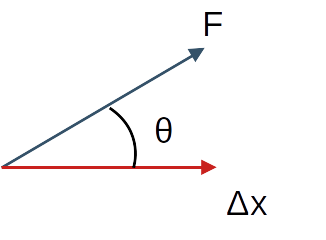
\includegraphics[scale=0.5]{work_angle.png}
\caption{Here is a force and displacement separated by an angle of $\theta$. Only the component of force along the displacement does work.}
\label{work_angle}
\end{figure}

\begin{exampleblock}

Yvonne pulls a box along the floor by exerting a force of $70.0 \, N$ at an angle of $50.0^{\circ}$ above horizontal. If she slides the box $6.50 \, m$, how much work does Yvonne do on the box?

\hspace{10pt}

We are given that $F = 70.0 \, N$, $\theta = 50.0^{\circ}$, and $\Delta x = 6.5 \, m$. The work done is

\begin{equation}
W = (70.0 \, N) (6.5 \, m) \, cos(50.0^{\circ}) = 292 \, J
\end{equation}

She does $W = 292 \, J$ of work on the box.

\end{exampleblock}

\section{Gravitational Potential Energy}

We are going to give special consideration to the work done by gravity on an object. Let's define up as positive, meaning that the force of gravity acting on an object of mass $m$ is

\begin{equation}
F_g = -mg
\end{equation}

This means that the work done by gravity as an object changes height by $\Delta y$ is

\begin{equation}
W_g = -mg \Delta y
\end{equation}

\begin{exampleblock}

Terry throws a rock straight up in the air so it reaches its maximum height at $3.5 \, m$ above where they threw it. Use the work-kinetic energy theorem to find the velocity Terry threw the rock at.

\hspace{10pt}

We know that $\Delta y = 3.5 \, m$ and the final velocity is $v_f = 0 \, \frac{m}{s}$. Lets start with the work-kinetic energy theorem.

\end{exampleblock}

We can check that this holds true even for objects that don't move just vertically. For example, we will look at a block sliding down a ramp in Figure \ref{gravramp}. The block slides down the ramp, changing its position by $d$. The height of the ramp is $h$ and the angle at the top of the ramp is $\theta$. Defining up as positive, we can write the work done by gravity as 

\begin{equation}
W_g = -mg \cdot (-d \, cos(\theta)) = mg \, cos(\theta)
\end{equation}

The height of the ramp is the adjacent side of the triangle from the angle $\theta$.

\begin{equation}
h = d \, cos(\theta)
\end{equation}

This means we can write the work done by gravity as

\begin{equation}
W_g = mgh
\end{equation}

Which means that the work only depends on the vertical movement. Note that the work is positive because the block moves downward, which is in the direction of the force of gravity.

\begin{figure}[t]
\centering
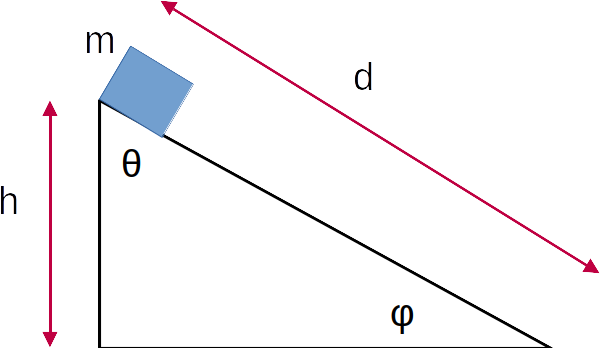
\includegraphics[scale=0.3]{gravity_ramp.png}
\caption{A block slides down a ramp of length $d$, changing its vertical position by $-h$. The angle at the top of the ramp is $\theta$.}
\label{gravramp}
\end{figure}

Since gravity from the Earth plays a role in all motion at the Earth's surface, we account for this by describing the work gravity can do with \textbf{gravitational potential energy}. An object of mass $m$ at a height of $h$ has a gravitational potential energy of

\begin{equation}
PE_g = mgh
\end{equation}

It is often easier to think about gravitational potential energy rather than the work done be energy, which we will see shortly. When we introduce potential energy, doing work on an object can change both kinetic energy and potential energy.

\begin{equation}
W = \Delta KE + \Delta PE
\end{equation}

\begin{exampleblock}

Kevin sees a book on the floor and picks it up to put on a shelf. The book has a mass of $0.30 \, kg$ and the shelf is $1.9 \, m$ above the floor. How much work does Kevin do on the book?

\hspace{10pt}

Let's define the floor as height $0 \, m$, so the shelf is at a height of $1.9 \, m$. The book as at rest in both the final and initial state, so $v_i = v_f = 0 \, \frac{m}{s}$. This means that $\Delta KE = 0 \, J$, so we have

\begin{equation}
W = \Delta PE = PE_f - PE_i
\end{equation}

\begin{equation}
W = mgh_f - mgh_i
\end{equation}

The book starts on the floor, which we defined as having a height of zero.

\begin{equation}
W = (0.30 \, kg) (9.8 \, \frac{m}{s^2}) (1.9 \, m) = 5.6 \, J
\end{equation}

Kevin does $W = 5.6 \, J$ of work on the book.

\end{exampleblock}

\section{Elastic Forces}

I am going to guess that everybody reading this has stretched a rubber band before. What did you notice about the band while you were pulling on it? Observations may include:

\begin{itemize}
\item The rubber band pulls back against your hand.
\item You have to pull harder the further you stretch the rubber band.
\item The rubber band will return to its original size and shape.
\end{itemize}

These are all characteristics of an \textbf{elastic force}. Elastic forces are exerted by objects that are stretched or compressed and try to return to their original shape. This includes rubber bands, tennis balls (they compress when they bounce), and the classic physics example of a spring. The force exerted by an ideal spring is stated by Hooke's Law (named after Robert Hooke, who studied springs)

\begin{equation}
F_e = -k \Delta x
\label{hooke}
\end{equation}

where $k$ is the spring constant and $x$ is how far the spring is stretched or compressed from equilibrium. There is a lot going on here, so let's look at this in detail.

\begin{figure}[H]
\centering
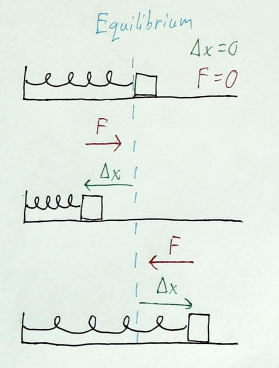
\includegraphics[scale=0.7]{spring_intro.png}
\caption{The force of a spring is exerted in the opposite direction of its displacement.}
\label{springintro}
\end{figure}

The \textbf{spring constant} is a measure of the stiffness of a spring. The units are $\frac{force}{length}$, and is typically in $\frac{N}{m}$ or $\frac{N}{cm}$ depending on the spring. A greater spring constant means the spring is stiffer and will have more resistance to being stretched or compressed. The spring constant of each spring is different and it depends on the shape and construction of the spring.

We know that $\Delta x$ is a displacement, but we need to know what it is a displacement relative to. Hooke's Law needs the displacement away from the \textbf{equilibrium length} of the spring. The equilibrium length is the spring's natural resting length, where it does not exert a force. This means that the force is stronger the further from the equilibrium length the spring is stretched or compressed. That is why it felt like you had to pull harder on the rubber band the further you stretched it.

The last thing of note from Hooke's Law is the negative sign, which indicates the force is exerted in the opposite direction that the spring is displaced. The elastic force is a type of \textbf{restoring force} because it acts to restore the spring to its original shape.

\begin{exampleblock}

A spring with spring constant $60.0 \, \frac{N}{cm}$ is compressed by a distance of $1.50 \, cm$ to the left. What is the magnitude and direction of the force?

\hspace{10pt}

Define right as positive. Since our spring is compressed to the left, that makes the displacement negative. We are given values of $k = 60 \, \frac{N}{cm}$ and $\Delta x = - 1.50 \, cm$. We can use Hooke's Law  now

\begin{equation}
F_e = -k \Delta x = -(60.0 \, \frac{N}{cm}) \cdot (-1.50 \, cm) = 90.0 \, N
\end{equation}

The force has a magnitude of $90.0 \, N$. We find that $F_e$ is positive, so the force is directed to the right. That makes sense for the displacement being to the left, since the elastic force is a restoring force.

\end{exampleblock}

\begin{exampleblock}

A spring is hanging vertically from the ceiling. When a $12.0 \, kg$ mass is attached the spring, the spring stretches downward by $5.50 \, cm$. What is the spring constant of the spring in $\frac{N}{m}$?

\begin{figure}[H]
\centering
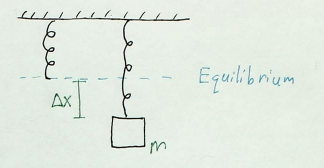
\includegraphics[scale=1.0]{spring_weight.png}
\caption{A spring is stretched downward by the force of gravity from an attached mass.}
\label{springweight}
\end{figure}

\hspace{10pt}

 Define up as positive, so the force of gravity is negative and $\Delta x = -5.50 \, cm$. We will convert the displacement to meters because we are asked to give the spring constant in $\frac{N}{m}$.

\begin{equation}
\Delta x = -5.50 \, cm \cdot \frac{1 \, m}{100 \, cm} = -0.0550 \, m
\end{equation}

This is a helpful problem to draw a free body diagram. We can see that the block is stationary only if the sum of the force of gravity and the elastic force is zero.

\begin{equation}
F_{net} = F_e + F_g = 0
\end{equation}

\begin{equation}
F_e = -k \Delta x
\end{equation}

\begin{equation}
F_g = -mg
\end{equation}

\begin{equation}
-k \Delta x - mg = 0
\end{equation}

\begin{equation}
k = \frac{-mg}{\Delta x} = \frac{-(12.0 \, kg) (9.8 \, m/s^2)}{(-0.0550 \, m)} = 2140 \, \frac{N}{m}
\end{equation}

The spring constant is $k = 2140 \, \frac{N}{m}$.

\end{exampleblock}

While we did talk extensively about about springs, Hooke's Law is a good approximation for many elastic objects at small deformations. 

\section{Elastic Potential Energy}

From the example with a block hanging from a vertical spring, let's look at the force that somebody would have to apply to a spring to displace it by a certain amount. Since the force exerted by a spring is $F_e = -k \Delta x$, you have to apply a force of $F_{app} = k \Delta x$ to displace it by $\Delta x$. This means the net force is zero at $\Delta x$ and the spring will be stationary. Let's see this visually in Figure \ref{fspring}.

\begin{figure}[H]
\centering
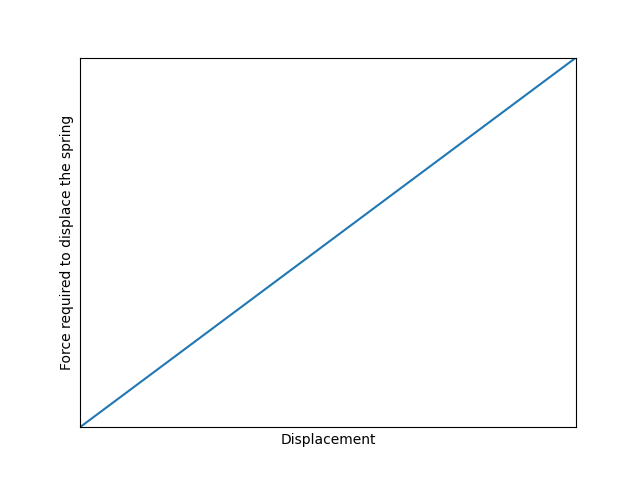
\includegraphics[scale=0.6]{force_spring.png}
\caption{The force required to displace a spring increases linearly with displacement.}
\label{fspring}
\end{figure}

We know that for a constant force the work is $W = F \Delta x \, cos(\theta)$, but here the force isn't constant. With a varying force we can find work by finding the area under the curve of a \textit{Force vs. Displacement} graph. This is very similar to how we found the displacement as the area under the graph of a \textit{v vs. t} plot. Looking at Figure \ref{fspring}, the area under the curve is a right triangle with base $\Delta x$ and height $F = k \Delta x$. The area of a triangle is

\begin{equation}
A = \frac{b \cdot h}{2}
\end{equation} 

\begin{equation}
W = \frac{\Delta x \cdot k \Delta x}{2} = \frac{1}{2}k (\Delta x)^2
\end{equation}

This is the amount of work required to displace the spring by $\Delta x$. Similar to how lifting an object converts work into gravitational potential energy, we can think of this work being converted to \textbf{elastic potential energy}.

\begin{equation}
PE_e = \frac{1}{2} k (\Delta x)^2
\end{equation}

This is the potential energy stored in a spring of spring constant $k$ displaced by $\Delta x$. We can't use kinematics to study the motion of an object on a spring (since acceleration varies), but work and energy makes it possible!

\begin{exampleblock}

How much potential energy is stored in a spring of spring constant $k = 40.0 \, \frac{N}{cm}$ that is compressed by $\Delta x = 3.50 \, cm$? 

\hspace{10pt}

We want to find the energy in units of Joules, so we will convert all of the $cm$ to $m$ so that we can get $N \cdot m = J$ as our unit at the end.

\begin{equation}
40.0 \frac{N}{cm} \cdot \frac{100 \, cm}{1 \, m} = 4000 \, \frac{N}{m}
\end{equation}

\begin{equation}
3.50 \, cm	\cdot \frac{1 \, m}{100 \, cm} = 0.0350 \, m
\end{equation}

Now we can plug in our values to find the elastic potential energy.

\begin{equation}
PE_e = \frac{1}{2} (4000 \, \frac{N}{m}) (0.0350 \, m)**2 = 2.45 \, J
\end{equation}

The spring has $PE_e = 2.45 \, J$ of potential energy stored.

\end{exampleblock}

\section{Conservation of Energy} 

Now that we have defined kinetic energy and a couple different types of potential energy, we are ready to look at the \textbf{Law of Conservation of Energy}.

\linespace

\textbf{The law of conservation of energy states that energy cannot be created or destroyed. It can be transferred between objects and/or transformed from one type of energy to another, but the total amount of energy remains constant.}

\linespace

This gives us a new way to think about potential energy: the potential of an object to move as the potential energy is converted to kinetic energy. A falling rock is constantly having its gravitational potential energy converted to kinetic energy. While it is falling, its downward velocity is increasing, which means its kinetic energy is increasing.

When there is no external work being done on an object, we can write

\begin{equation}
E_{initial} = E_{final}
\end{equation}

Since we will look at how energy is transformed between types, we can write this using kinetic and potential energy.

\begin{equation}
KE_i + PE_i = KE_f + PE_f
\label{econs}
\end{equation}

Equation \ref{econs} is the main mathematical model for looking at conservation of energy. It says that the sum of kinetic and potential energy is the same in the initial and final state when there is is no external work done on the objected. (We will look at external work in the next section.)

One consequence is that conservation of energy is \textbf{path-independent}. That means we don't need to worry about what happens between the initial and final state, just what those two states are like. The exact movement path and time required to change states does not come into the solution at all!

\begin{exampleblock}

A roller coaster just barely makes it over the first hill, which has a height of 75.0 $m$. If we treat the coaster as stationary at the top of the first hill, how fast is it moving at the top of the 60.0 $m$ tall second hill?

\hspace{10pt}

The initial state has the coaster at a height of $h_i = 75.0 \, m$ and velocity of $v_i = 0 \, \frac{m}{s}$. The final state has a height of $h_f = 60.0 \, m$ and an unknown $v_f$, which we are solving for.

Our energy terms are:

\begin{itemize}
\item $KE_i = \frac{1}{2} m v_i^2 = 0 \, \frac{m}{s}$
\item $PE_i = mgh_i$
\item $KE_f = \frac{1}{2} m v_f^2$
\item $PE_f = mgh_f$
\end{itemize}

Now we can use Equation \ref{econs}

\begin{equation}
KE_i + PE_i = KE_f + PE_f
\end{equation}

\begin{equation}
mgh_i = \frac{1}{2} m v_f^2 + mgh_f
\end{equation}

\begin{equation}
mg(h_i - h_f) = \frac{1}{2} m v_f^2
\end{equation}

\begin{equation}
v_f^2 = 2g(h_i - h_f)
\end{equation}

Notice how mass cancels out entirely! This is why we didn't need the mass of the roller coaster car.

\begin{equation}
v_f = \sqrt{2g(h_i - h_f)}
\end{equation}

\begin{equation}
v_f = \sqrt{2(9.8 \, m/s^2) (75.0 \, m - 60.0 \, m} = 17.1 \, \frac{m}{s}
\end{equation}

The roller coaster is moving at $v_f = 17.1 \, \frac{m}{s}$ at the top of the second hill.

\end{exampleblock}

\begin{exampleblock}

A block of mass $1.75 \, kg$ slides down a ramp angled at $30.0^{\circ}$ above horizontal. The block starts at rest at a height of $1.20 \, m$. When it reaches the bottom of the ramp, the block hits a spring and compresses it by $4.00 \, cm$ before coming to a stop. What is the spring constant of the spring?

\begin{figure}[H]
\centering
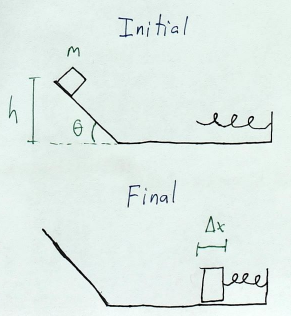
\includegraphics[scale=0.8]{spring_ramp_conservation.png}
\caption{The block starts at the top of a ramp, then slides down and compresses a spring until the block stops moving.}
\label{springramp}
\end{figure}

\hspace{10pt}

In the initial state the block has gravitational potential energy determined by its height, and in the final state the spring has elastic potential energy since it is compressed by the block. In both states the block is stationary, so despite the fact that the block slid from one position to another there is no kinetic energy in the initial or final state.

Our known values are:

\begin{itemize}
\item $v_i = v_f = 0 \, \frac{m}{s}$
\item $m = 1.75 \, kg$
\item $h_i = 1.20 \, m$
\item $\Delta x_f = 4.00 \, cm = 0.0400 \, m$
\end{itemize}

The angle of the ramp has no effect on the on the gravitational potential energy or the conservation of energy, so we don't need to use that information. Our energy terms are:

\begin{itemize}
\item $KE_i = KE_f = 0 \, J$
\item $PE_i = mgh_i$
\item $PE_f = \frac{1}{2} k (\Delta x_f)^2$
\end{itemize}

\begin{equation}
mgh_i = \frac{1}{2} k (\Delta x_f)^2
\end{equation}

\begin{equation}
k = \frac{1}{(\Delta x_f)^2} \cdot 2mgh_i
\end{equation}

\begin{equation}
k = \frac{1}{(0.0400 \, m)^2} \cdot 2 (1.75 \, kg) (9.8 \, \frac{m}{s^2} (1.2 \, m) = 25700 \, \frac{N}{m}
\end{equation}

The spring constant is $k = 25700 \, \frac{N}{m}$.

\end{exampleblock}

\section{External Work and Nonconservative Forces}

In the previous section we used conservation of energy to study scenarios where there was no external work being done on an object. Here we will use energy to see that energy can still be used even with external work.

When external work is done on a system, that work changes one or both of the kinetic energy or potential energy. As an equation, this is

\begin{equation}
W_{ext} = \Delta KE + \Delta PE
\label{dME}
\end{equation}

The sum of the kinetic and potential energy is a quantity that we call the \textbf{mechanical energy}.

\begin{equation}
Mechanical \, Energy = KE + PE
\end{equation}

External work on a system changes the mechanical energy. In the previous section, the mechanical energy was constant because there was no external work. Even though the mechanical energy changes, total energy is still conserved because the external work requires energy to do. For example, if the external work is you pushing a box, chemical potential energy from the food you have eaten is used to do they work. Returning to Equation \ref{dME}, we can write

\begin{equation}
W_{ext} = KE_f - KE_i + PE_f - PE_i
\end{equation}

\begin{equation}
KE_i + PE_i + W_{ext} = KE_f + PE_f
\label{wext}
\end{equation}

The mechanical energy in the final state is the mechanical energy in the initial state plus the external work done.

\begin{exampleblock}

A subway train uses a spring to help it stop at the end of the track. The train has a mass of 9000 $kg$ and approaches the end of the track moving at 18.0 $\frac{m}{s}$. If the $k = 45,000,000 \, \frac{N}{m}$ spring should be compressed by no more than 25.0 $cm$ when the train stops, how much work do the brakes need to do on the train to slow it down?

\hspace{10pt}

We want to solve for $W_{ext}$, so let's take stock of what we know and our energy terms.

\begin{itemize}
\item $m = 9000 \, kg$
\item $v_i = 18.0 \, \frac{m}{s}$
\item $k = 45,000,000 \, \frac{N}{m}$
\item $\Delta x_f = 25.0 \, cm = 0.250 \, m$
\item $KE_i = \frac{1}{2} m v_i^2$
\item $PE_f = \frac{1}{2} k (\Delta x_f)^2$
\item $KE_f = PE_i = 0 \, J$
\end{itemize}

This gives us

\begin{equation}
\frac{1}{2} m v_i^2 + W_{ext} = \frac{1}{2} k (\Delta x)^2
\end{equation}

\begin{equation}
W_{ext} = \frac{1}{2} (k (\Delta x)^2 - m v_i^2) = -51,800 \, J
\end{equation}

The brakes would need to do $W_{ext} = -51,800 \, J$ of work on the train. A negative external work means that the final state has less energy than the initial state, which makes sense because the train has to slow down so it doesn't compress the spring too far.

\end{exampleblock}

As in the example above, many times we will see a negative external work that reduces the mechanical energy of the system. Friction and air resistance are two common sources of negative work on a system. Both of these forces are \textbf{nonconservative forces}, meaning that they do not allow for kinetic energy to be stored as kinetic energy. Instead, the kinetic energy is dissipated in the environment as \textbf{thermal energy} which \textit{cannot} be converted back to kinetic energy. Thermal energy commonly includes heat and sound, both of which you will observe with friction. Surfaces that slide along each other will heat up and produce a sound as they scrape or slide.

Nonconservative forces introduce a path-dependence to motion that we don't see with conservation of energy. For example, if there is friction between a block and a table, the further the block slides on the table the more external work is done and the lower the final energy will be. If there is no external work, analyzing motion with energy is path-independent and we only look at the initial and final states.

\section{Power}

So far we have been able to completely ignore time when studying work and energy. However, it is sometimes useful to look at energy transfer over time. \textbf{Power} is a measure of energy transfer per unit of time. It is abbreviated $P$.

\begin{equation}
P = \frac{\Delta E}{\Delta t}
\label{power}
\end{equation}

 The SI unit of power is the \textbf{Watt}, which is abbreviated $W$.

\begin{equation}
1 \, Watt = \frac{1 \, Joule}{1 \, second}
\end{equation}

Power tells us how quickly an object changes its kinetic and/or potential energy. It is the difference in a car going from 0 to 60 $mph$ in 5 seconds vs. 2 seconds. Both are the same change in kinetic energy, but the time required is different so the power required of the engine are different.

\begin{exampleblock}

Joseph is hiking and after 2 hours finds himself at the top of a 300 meter tall hill. If his mass is 70.0 $kg$, how much power did he exert climbing the hill?

\hspace{10pt}

Here we know his mass $m = 70.0 \, kg$, his change in height is $\Delta h = 300 \, m$, and the time is $\Delta t = 2 \, hrs$. First let's convert the time to seconds.

\begin{equation}
2 \, hrs \cdot \frac{60 \, min}{1 \, hr} \cdot \frac{60 \, s}{1 \, min} = 7200 \, s
\end{equation}

The change in his energy is the change in his gravitational potential energy based on height.

\begin{equation}
\Delta E = mg \Delta h
\end{equation}

\begin{equation}
P = \frac{mg \Delta h}{\Delta t} = \frac{(70.0 \, kg) (9.8 \, m/s^2) (300 \, m)}{7200 \, s} = 28.6 \, W
\end{equation}

Joseph has to exert a power of $P = 28.6 \, W$ while hiking up the hill.

\end{exampleblock}


\chapter{Momentum, Impulse, and Collisions}
\setcounter{example}{1}
\addtocounter{chp}{1}

Consider a tennis ball that is dropped and bounces back up from the floor. The ball undergoes a rapid change in velocity when it hits the floor. This is not a practical problem to approach with work because the force isn't being exerted over some distance. Kinematics also aren't suitable because the bounce may not have constant acceleration. We need a new approach to address scenarios like this.

\begin{figure}[H]
\centering
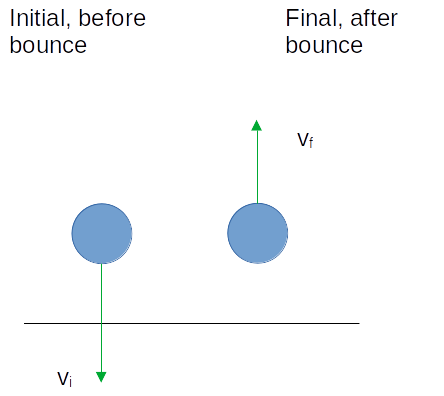
\includegraphics[scale=0.4]{bounce.png}
\caption{The velocities of a falling ball before and after a bounce. This change in velocity happens during the short time the ball is in contact with the ground.}
\label{bounceground}
\end{figure}

\section{Momentum and Impulse}

First we will need to define some new quantities for modeling a rapid change in velocity. To do this we will start with Newton's 2nd Law of Motion

\begin{equation}
F_{net} = ma
\end{equation}

From the definition of acceleration, we will write it as change in velocity divided by change in time.

\begin{equation}
F_{net} = m \frac{\Delta v}{\Delta t}
\end{equation}

Multiply both sides by $\Delta t$.

\begin{equation}
F_{net} \, \Delta t = m \, \Delta v
\label{momimp}
\end{equation}

Let's first look at the right hand side of Equation \ref{momimp}. The product of mass times velocity is a quantity called \textbf{momentum}, which is abbreviated $p$.

\begin{equation}
p = mv
\label{momdef}
\end{equation}

The units of momentum are just the product of mass and velocity units, so $\frac{kg \, m}{s}$. Momentum is a measure of motion that takes into account ``how big and how fast'' the object moving is. Two objects can have the same momentum with very different velocities if the masses are different.

If we write out the change in momentum, it would be

\begin{equation}
\Delta p = \Delta m \, v + m \, \Delta v
\end{equation}

We are looking at objects with fixed mass, so $\Delta m = 0 \, kg$. Therefore, the change in momentum is just $m \, \Delta v$. (If you have taken calculus, you might recognize the above equation as an application of the product rule of derivatives.)

So the right hand side of Equation \ref{momimp} is the change in momentum. What about the left hand side? Force times the time interval is a quantity called \textbf{impulse}, which is abbreviated as $J$. Be careful to not confuse this with the unit Joule, as both are abbreviated $J$. 

The impulse due to a force $F$ is

\begin{equation}
J = F \, \Delta t
\label{impdef}
\end{equation}

The units are the units of force times time. Let's start with $Newton \cdot second$ and simplify.

\begin{equation}
N \cdot s = \frac{kg \, m}{s^2} \cdot s = \frac{kg \, m}{s}
\end{equation}

Notice that this is the same unit as momentum! This is important, since we see from Equation \ref{momimp} the impulse is equal to the change in momentum.

\begin{equation}
J = \Delta p = p_f - p_i = m v_f - m v_i
\label{impulse}
\end{equation}

Now we have an approach to study fast changes in velocity by finding the change in momentum and using impulse!

\begin{exampleblock}

A tennis ball is dropped onto the floor. Right before it hits the ground, it is moving downward at 6.00 $\frac{m}{s}$. After it bounces, it is moving upward at 4.80 $\frac{m}{s}$. The mass of a tennis ball is 58.0 $g$. This is the same scenario we saw in Figure \ref{bounceground}.


\begin{enumerate}
\item What impulse does the floor exert on the tennis ball?
\item If a high speed camera shows the ball is in contact with the floor for 0.015 $s$, what is the average force the floor exerts on the ball?
\end{enumerate}

\hspace{10pt}

\begin{enumerate}
\item First we will define up as positive. We have $v_i = -6.00 \, \frac{m}{s}$, $v_f = 4.80 \, \frac{m}{s}$, and $m = 58.0 \, g = 0.0580 \, kg$. The impulse can be found with equation \ref{impulse}.

\begin{equation}
J = m v_f - m v_i 
\end{equation}

\begin{equation}
J = 0.0580 \, kg \cdot (4.80 \, \frac{m}{s} - (-6.00) \, \frac{m}{s}) = 0.626 \, \frac{kg \, m}{s}
\end{equation}

The impulse is $J = 0.626 \, \frac{kg \, m}{s}$. This value is positive, so it is directed upward.

\item Now we are told the time of impact with the floor has been measured at $\Delta t = 0.0150 \, s$. Using Equation \ref{impdef}

\begin{equation}
J = F \, \Delta t
\end{equation}

\begin{equation}
F = \frac{J}{\Delta t} = \frac{0.626 \, kg \, m/s}{0.015 \, s} = 41.8 \, N
\end{equation}

The average force the floor exerts on the ball is $F = 41.8 \, N$.
\end{enumerate}

\end{exampleblock}

\section{Conservation of Momentum}

Newton's 3rd Law has an interesting consequence for momentum. Remember that the law states that if object A exerts a force on object B, then object B exerts a force on object A that is of equal magnitude and opposite direction. What does that mean for impulse? The the forces between two objects will be exerted for the same duration of time, so the impulses will also be equal magnitude and opposite direction. 

\begin{equation}
J_A = -J_B
\end{equation}

This means that their change in momenta will also be equal in magnitude and opposite in direction.

\begin{equation}
\Delta p_A = -\Delta p_B
\end{equation}

This means that for objects A and B that exert an impulse on each other, \textit{the total momentum of both objects does not change.} This is called the \textbf{Law of Conservation of Momentum}.

\linespace

\textbf{The law of conservation of momentum states any interaction of two objects will not change the total momentum of the two objects in the system. The momentum of each object can change but the total momentum is constant.}

\linespace

No change in momentum happens on its own, it is always ``balanced'' by a change in momentum of another object. How does this work if you are pushing a box along the floor but not sliding backward? Friction between your feet and the floor keeps you from sliding by exerting a force between you and the floor. The Earth will experience the change in momentum, but its mass so large that motion can be safely ignored.

\begin{exampleblock}

Sarah and Valerie are on a frozen lake and decide to test out conservation of momentum. They start at rest and then push off from each other. Sarah slides to the right at 2.0 $\frac{m}{s}$. If Sarah has a mass of 60.0 $kg$ and Valerie has a mass of 52.0 $kg$, how fast would we expect Valerie to slide?

\hspace{10pt}

Define right as positive. Both people start at rest, so the final momentum of each one is equal to their change in momentum. From conservation of momentum we have

\begin{equation}
\Delta p_S = -\Delta p_V
\end{equation}

We are given $m_S = 60.0 \, kg$, $m_V = 52.0 \, kg$, $v_S = 2.0 \, \frac{m}{s}$. 

\begin{equation}
m_S v_S = -m_V v_V 
\end{equation}

\begin{equation}
v_V = \frac{-m_S v_S}{m_V} = \frac{-(60.0 \, kg)(2.0 \, m/s)}{52 \, kg} = -2.3 \, \frac{m}{s}
\end{equation}

Valerie has a velocity of $v_V = -2.3 \, \frac{m}{s}$, so she is moving to the left at a speed of 2.3 $\frac{m}{s}$.

\end{exampleblock}

\section{Perfectly Inelastic Collisions}

Collisions between 2 objects are perfect for study with conservation of momentum. If we know the momentum of the objects before they collide, we know what the total momentum is after the collision. That will let us determine the velocity of the objects after the collision.

The first type of collision we will study are \textbf{perfectly inelastic collisions}, in which the two objects that collide stick together. This results in the maximum loss of kinetic energy, as energy goes into deforming the objects so they stick together. This could happen if two clay balls collide and stick together. 

Mathematically we will look at objects 1 and 2 with masses $m_1$ and $m_2$ that have initial velocities $v_{1,i}$ and $v_{2,i}$ before the collision. After the collision, the objects are stuck together moving at final velocity $v_f$. 

\begin{equation}
p_i = m_1 v_{1,i} + m_2 v_{2,i}
\end{equation}

\begin{equation}
p_f = (m_1 + m_2) v_f
\end{equation}

The final momentum has the sum of the masses because the two objects are stuck together, so their total mass is moving at $v_f$. Now we can use conservation of momentum to write.

\begin{equation}
m_1 v_{1,i} + m_2 v_{2,i} = (m_1 + m_2) v_f
\label{inelastic}
\end{equation}

We figure out the direction the two objects move after the collision from the sign of the final velocity. We need to define a direction as positive and give our initial velocities the correct signs. Then, when we solve the problem the sign of the final velocity will tell us the direction the objects move.

\begin{exampleblock}

Two carts approach each other on a track. Both have magnets so that they will stick together when they collide. Cart 1 has a mass of $0.80 \, kg$ and is moving to the right at $2.0 \, \frac{m}{s}$. Cart 2 has a mass of $1.6 \, kg$ and is moving to the left at $1.5 \, \frac{m}{s}$. After the carts collide, what is their velocity? Make sure to specify magnitude and direction.

\hspace{10pt}

Define right as positive. We are given

\begin{itemize}
\item $m_1 = 0.80 \, kg$
\item $v_{1,i} = 2.0 \, \frac{m}{s}$
\item $m_2 = 1.6 \, kg$
\item $v_{2,i} = -1.5 \, \frac{m}{s}$
\end{itemize}

Since cart 2 is moving left, it has a negative velocity. Now we can use Equation \ref{inelastic}.

\begin{equation}
m_1 v_{1,i} + m_2 v_{2,i} = (m_1 + m_2) v_f
\end{equation}

\begin{equation}
v_f = \frac{m_1 v_{1,i} + m_2 v_{2,i}}{m_1 + m_2}
\end{equation}

\begin{equation}
v_f = \frac{(0.80 \, kg)(2.0 \, m/s) + (1.6 \, kg)(-1.5 \, m/s)}{2.4 \, kg} = -0.33 \, \frac{m}{s}
\end{equation}

The two carts are moving to the left, having a velocity of $v_f = -0.33 \, \frac{m}{s}$.

\end{exampleblock}

\begin{exampleblock}

Artemis is at the range practicing her archery. She shoots an arrow into a box, causing the box to slide backward. The arrow has a mass of $0.0165 \, kg$ and hits the box at a velocity of $90.0 \, \frac{m}{s}$. The arrow sticks in the box, causing the box to slide at a velocity of $25.0 \, \frac{cm}{s}$. What is the mass of the box. (Note that the box is initially stationary.)

\hspace{10pt}

This may not seem like a collision, but since the arrow sticks in the box this is a perfectly inelastic collision. We will take stock of our known values. The arrow is object 1 and box is object 2.

\begin{itemize}
\item $m_1 = 0.0165 \, kg$
\item $v_{1,i} = 90.0 \, \frac{m}{s}$
\item $v_{2,i} = 0 \, \frac{m}{s}$
\item $v_{f} = 25.0 \, \frac{cm}{s} = 0.25 \, \frac{m}{s}$
\end{itemize}

Now we can use Equation \ref{inelastic} to solve for $m_2$

\begin{equation}
m_1 v_{1,i} + m_2 v_{2,i} = (m_1 + m_2) v_f
\end{equation}

We can simplify this by plugging in $v_{2,i} = 0$.

\begin{equation}
m_1 v_{1,i} = m_1 v_f + m_2 v_f
\end{equation}

\begin{equation}
m_1 (v_{1,i} - v_f) = m_2 v_f
\end{equation}

\begin{equation}
m_2 = m_1 \left( \frac{v_{1,i}}{v_f} - 1 \right)
\end{equation}

\begin{equation}
m_2 = 0.0165 \, kg \cdot \left( \frac{90.0 \, m/s}{0.25 \, m/s} - 1 \right) = 5.92 \, kg
\end{equation}

The box has a mass of $m_2 = 5.92 \, kg$.

\end{exampleblock}

\section{Perfectly Elastic Collision}

As we know from life experience, not all objects stick together when they collide. One example that comes to mind is the collision of the cue ball with another ball when playing pool. In general this is difficult to study and requires detailed knowledge about the composition of the objects. However, we can make another very useful approximation to further our studies. We can model some collisions as \textbf{perfectly elastic collisions}, where kinetic energy is conserved before and after the collision. This is in stark contrast with perfectly inelastic collisions, where kinetic energy is converted to thermal energy in the process of making the two objects stick together.

Mathematically this requires a different treatment because both objects are moving independently after the collision. Therefore we do not have a single $v_f$ for both but need to consider $v_{1,f}$ and $v_{2,f}$ for objects 1 and 2, respectively. If those objects have masses $m_1$ and $m_2$, and are moving at velocities $v_{1,i}$ and $v_{2,i}$ before the collision, we can write conservation of momentum as

\begin{equation}
m_1 v_{1,i} + m_2 v_{2,i} = m_1 v_{1,f} + m_2 v_{2,f}
\label{elasticmom}
\end{equation}

Even if we know the full initial state before the collision, we now have two unknowns in the two final velocities. To solve this, we need to use conservation of kinetic energy as well.

\begin{equation}
\frac{1}{2} m_1 v_{1,i}^2 + \frac{1}{2} m_2 v_{2,i}^2 = \frac{1}{2} m_1 v_{1,f}^2 + \frac{1}{2} m_2 v_{2,f}^2
\label{elasticenergy}
\end{equation}

Now we have a system of two equations and two unknowns, which we can solve for. An example of how to do so is shown below.

\begin{exampleblock}

Two carts with elastic bumpers collide on a track in a perfectly elastic collision. Cart 1 has a mass of $0.80 \, kg$ and is moving to the right at $2.0 \, \frac{m}{s}$. Cart 2 has a mass of $1.6 \, kg$ and is moving to the left at $1.5 \, \frac{m}{s}$. What is the velocity of each cart after the collision? Be careful with signs so we know what direction each cart moves.

\hspace{10pt}

Choose right to be positive. We will take stock of our known values

\begin{itemize}
\item $m_1 = 0.80 \, kg$
\item $v_{1,i} = 2.0 \, \frac{m}{s}$
\item $m_2 = 1.6 \, kg$ 
\item $v_{2,i} = -1.5 \, \frac{m}{s}$
\end{itemize}

With Equations \ref{elasticmom} and \ref{elasticenergy} we have our system of two equations to find the two unknowns, $v_{1,f}$ and $v_{2,f}$. To start with, take Equation \ref{elasticmom} and solve it for one of the unknown velocities. Here we will do so for $v_{2,f}$.

\begin{equation}
m_1 v_{1,i} + m_2 v_{2,i} = m_1 v_{1,f} + m_2 v_{2,f}
\end{equation}

\begin{equation}
m_2 v_{2,f} = m_1 (v_{1,i} - v_{1,f}) + m_2 v_{2,i}
\end{equation}

\begin{equation}
v_{2,f} = \frac{m_1}{m_2} (v_{1,i} - v_{1,f}) + v_{2,i}
\end{equation}

Now we can plug this in for $v_{2,f}$ in Equation \ref{elasticenergy}.

\begin{equation}
\frac{1}{2} m_1 v_{1,i}^2 + \frac{1}{2} m_2 v_{2,i}^2 = \frac{1}{2} m_1 v_{1,f}^2 + \frac{1}{2} m_2 \left( \frac{m_1}{m_2}(v_{1,i} - v_{1,f}) + v_{2,i} \right)^2
\end{equation}

This looks like a mess, but we do know have $v_{1,f}$ as our only unknown. Let's try to solve for that.

\begin{equation}
m_1 v_{1,i}^2 + m_2 v_{2,i}^2 = m_1 v_{1,f}^2 + m_2 \left( \frac{m_1^2}{m_2^2}(v_{1,i}^2 - 2 v_{1,i} v_{1,f} + v_{1,f}^2) + 2 \frac{m_1}{m_2} (v_{1,i} v_{2,i} - v_{1,f} v_{2,i}) + v_{2,i}^2 \right)
\end{equation}

\begin{equation}
m_1 v_{1,i}^2 + m_2 v_{2,i}^2 = m_1 v_{1,f}^2 + \frac{m_1^2}{m_2} v_{1,i}^2 - 2 \frac{m_1^2}{m_2} v_{1,i} v_{1,f} + \frac{m_1^2}{m_2} v_{1,f}^2 + 2 m_1 v_{1,i} v_{2,i} - 2 m_1 v_{2,i} v_{1,f} + m_2 v_{2,i}^2
\end{equation}

If we want to look for a small upside, the $m_2 v_{2,i}^2$ terms cancel out. Keep plugging away. We will group up the terms that are linear in $v_{1,f}$ and terms that are quadratic in .

\begin{equation}
m_1 v_{1,i}^2 = \left( m_1 + \frac{m_1^2}{m_2} \right) v_{1,f}^2 + \frac{m_1^2}{m_2} v_{1,i}^2 + \left( -2 \frac{m_1^2}{m_2} v_{1,i} - 2 m_1 v_{2,i} \right) v_{1,f} + 2 m_1 v_{1,i} v_{2,i}
\end{equation}

\begin{equation}
0 = \left( m_1 + \frac{m_1^2}{m_2} \right) v_{1,f}^2 - 2 \left( \frac{m_1^2}{m_2} v_{1,i} + m_1 v_{2,i} \right) v_{1,f} + \left( \frac{m_1^2}{m_2} - m_1 \right) v_{1,i}^2 + 2 m_1 v_{1,i} v_{2,i}
\end{equation}

Now we have a quadratic equation in the form $0 = ax^2 + bx + c$, so we can solve for $v_{1,f}$ using the quadratic formula.

\begin{equation}
x = \frac{-b \pm \sqrt{b^2 - 4ac}}{2a}
\end{equation}

\begin{equation}
a = m_1 + \frac{m_1^2}{m_2} 
\end{equation}

\begin{equation}
b = -2 \left( \frac{m_1^2}{m_2} v_{1,i} + m_1 v_{2,i} \right)
\end{equation}

\begin{equation}
c = \left( \frac{m_1^2}{m_2} - m_1 \right) v_{1,i}^2 + m_1 v_{1,i} v_{2,i}
\end{equation}

To start with, let's work on $b^2 - 4ac$ that is in the radical.

\begin{equation}
b^2 = 4 \frac{m_1^4}{m_2^2} v_{1,i}^2 + 8 \frac{m_1^3}{m_2} v_{1,i} v_{2,i} + 4 m_1^2 v_{2,i}^2
\end{equation}

\begin{equation}
4ac = 4 \left( m_1 + \frac{m_1^2}{m_2} \right) \left[ \left( \frac{m_1^2}{m_2} - m_1 \right) v_{1,i}^2 + m_1 v_{1,i} v_{2,i} \right]
\end{equation}

\begin{equation}
4ac = 4 \frac{m_1^4}{m_2^2} v_{1,i}^2 - 4 m_1^2 v_{1,i}^2 + 4 m_1^2 v_{1,i}v_{2,i} + 4 \frac{m_1^3}{m_2} v_{1,i} v_{2,i}
\end{equation}

We see that there will be a couple terms that cancel and some terms get grouped up.

\begin{equation}
b^2 - 4ac = 8 m_1 v_{1,i}^2 + 4 m_1^2 v_{1,i} v_{2,i} \left( 1 + \frac{m_1}{m_2} \right)
\end{equation}

The quadratic formula gives us

\begin{equation}
v_{1,f} = \frac{2 \left(\frac{m_1^2}{m_2} v_{1,i} + m_1 v_{2,i} \right) \pm \sqrt{8 m_1 v_{1,i}^2 + 4 m_1^2 v_{1,i} v_{2,i} \left( 1 + \frac{m_1}{m_2} \right)}}{2 \left(m_1 + \frac{m_1^2}{m_2} \right)}
\end{equation}

The two answers to this are $1.23 \, \frac{m}{s}$ and $-1.89 \, \frac{m}{s}$ How do we know which is the actual value of $v_{1,f}$? Let's use both in the conservation of momentum to find $v_{2,f}$ and see which value makes physical sense.

\begin{equation}
v_{2,f} = \frac{m_1}{m_2} (v_{1,i} - v_{1,f}) + v_{2,i}
\end{equation}

If we plug in $1.23 \, \frac{m}{s}$, we get $-1.12 \, \frac{m}{s}$ for $v_{2,f}$. If we plug in $-1.89 \, \frac{m}{s}$, we get $0.445 \, \frac{m}{s}$ for $v_{2,f}$. Now we have to think about our signs. Positive is right, negative is left. Initially, cart 1 was moving to the right and cart 2 left. After they collide, we cannot have cart 1 still moving to the right and cart 2 still moving to the left. That would mean the carts passed through each other! From that, we know the final velocities are

\begin{equation}
v_{1,f} = -1.89 \, \frac{m}{s}
\end{equation}

\begin{equation}
v_{2,f} = 0.445 \, \frac{m}{s}
\end{equation}

After the collision, cart 1 moves to the left at $1.89 \, \frac{m}{s}$ and cart 2 moves to the right at $0.445 \, \frac{m}{s}$.

\end{exampleblock}

As we can see, generalized perfectly elastic collisions can be very time consuming to solve! As a result we will focus on scenarios where one object is initially at rest. We will denote object 2 as the stationary one, so that $v_{2,i} = 0 \, \frac{m}{s}$. We can see how this works in the example below.

\begin{exampleblock}

A cart with an elastic bumper approaches a second, stationary cart and they collide in a perfectly elastic collision. The moving cart has mass $0.80 \, kg$ and initial velocity $2.0 \, \frac{m}{s}$ to the right. The stationary cart has mass $1.6 \, kg$. What is the velocity of each cart after the collision?

\hspace{10pt}

Define right to be positive. The moving cart is cart 1 and the stationary cart is cart 2.

\begin{itemize}
\item $m_1 = 0.80 \, kg$
\item $v_{1,i} = 2.0 \, \frac{m}{s}$
\item $m_2 = 1.6 \, kg$
\item $v_{2,i} = 0 \, \frac{m}{s}$
\end{itemize}

Now we can write our conservation laws, but with $v_{2,i} = 0 \, \frac{m}{s}$ already plugged in.

\begin{equation}
m_1 v_{1,i} = m_1 v_{1,f} + m_2 v_{2,f}
\end{equation}

\begin{equation}
\frac{1}{2} m_1 v_{1,i}^2 = \frac{1}{2} m_1 v_{1,f}^2 + \frac{1}{2} m_2 v_{2,f}^2
\end{equation}

Now we can solve the momentum equation for $v_{2,f}$

\begin{equation}
v_{2,f} = \frac{m_1}{m_2}(v_{1,i} - v_{1,f})
\end{equation}

Now we can plug this into the energy equation

\begin{equation}
m_1 v_{1,i}^2 = m_1 v_{1,f}^2 + m_2 \left( \frac{m_1}{m_2} (v_{1,i} - v_{1,f}) \right)^2
\end{equation}

\begin{equation}
m_1 v_{1,i}^2 = m_1 v_{1,f}^2 + \frac{m_1^2}{m_2} v_{1,i}^2 - 2 \frac{m_1^2}{m_2} v_{1,i} v_{1,f} + \frac{m_1^2}{m_2} v_{1,f}^2
\end{equation}

Now we can group up terms that have the same power of $v_{1,f}$

\begin{equation}
0 = \left( m_1 + \frac{m_1^2}{m_2} \right) v_{1,f}^2 - 2 \frac{m_1^2}{m_2} v_{1,i} v_{1,f} +\left( \frac{m_1^2}{m_2} - m_1 \right) v_{1,i}^2
\end{equation}

Now we have a quadratic equation in the form $0 = ax^2 + bx + c$. We can solve for $v_{1,f}$ with the quadratic formula.

\begin{equation}
x = \frac{-b \pm \sqrt{b^2 - 4ac}}{2a}
\end{equation}

\begin{equation}
a = m_1 + \frac{m_1^2}{m_2} 
\end{equation}

\begin{equation}
b = -2 \frac{m_1^2}{m_2} v_{1,i}
\end{equation}

\begin{equation}
c = \left( \frac{m_1^2}{m_2} + m_1 \right) v_{1,i}^2
\end{equation}

First we will look at the $b^2 - 4ac$ under the radical.

\begin{equation}
b^2 = 4 \frac{m_1^4}{m_2^2} v_{1,i}^2
\end{equation}

\begin{equation}
4ac = 4 \left( \frac{m_1^2}{m_2} + m_1 \right) \left(\frac{m_1^2}{m_2} - m_1 \right) v_{1,i}^2
\end{equation}

\begin{equation}
4ac = 4 \frac{m_1^4}{m_2^2} v_{1,i}^2 - 4m_1^2 v_{1,i}^2
\end{equation}

\begin{equation}
b^2 - 4ac = 4 \frac{m_1^4}{m_2^2} v_{1,i}^2 - 4 \frac{m_1^4}{m_2^2} v_{1,i}^2 + 4m_1^2 v_{1,i}^2
\end{equation}

\begin{equation}
b^2 - 4ac = 4 m_1^2 v_{1,i}^2
\end{equation}

Now we can look at the entire quadratic formula

\begin{equation}
v_{1,f} = \frac{2 \frac{m_1^2}{m_2} v_{1,i} \pm \sqrt{4 m_1^2 v_{1,i}^2}}{2 \left( \frac{m_1^2}{m_2} + m_1 \right)}
\end{equation}

\begin{equation}
v_{1,f} = \frac{2 \frac{m_1^2}{m_2} v_{1,i} \pm 2 m_1 v_{1,i}}{2 m_1 \left(\frac{m_1}{m_2} + 1 \right)}
\end{equation}

\begin{equation}
v_{1,f} = \frac{\frac{m_1}{m_2} \pm 1}{\frac{m_1}{m_2} + 1} v_{1,i}
\end{equation}

The plus-minus means we have 2 solutions from the equation, so let's see which makes sense for $v_{1,f}$. If we choose plus, then we get $v_{1,f} = v_{1,i}$. No collision happened at all! This is not the solution we want for the scenario we are studying. Therefore, the solution we want for the final velocity is

\begin{equation}
v_{1,f} = \frac{\frac{m_1}{m_2} - 1}{\frac{m_1}{m_2} + 1} v_{1,i}
\end{equation}

\begin{equation}
v_{1,f} = \frac{\frac{0.80 \, kg}{1.6 \, kg} - 1}{\frac{0.80 \, kg}{1.6 \, kg} + 1} \cdot 2.0 \, \frac{m}{s} = -0.67 \, \frac{m}{s}
\end{equation}

Now we can use the momentum equation to find the velocity of cart 2.

\begin{equation}
v_{2,f} = \frac{0.80 \, kg}{1.6 \, kg} (2.0 \, \frac{m}{s} - (-0.67 \, \frac{m}{s})) = 1.34 \, \frac{m}{s}
\end{equation}

Cart 1 will move to the left at $0.67 \, \frac{m}{s}$ and cart 2 will move to the right at $1.34 \, \frac{m}{s}$.

\end{exampleblock}

The equations we used in the above example can be applied to any elastic collision where object 2 is at rest in the initial state.

\begin{equation}
v_{1,f} = \frac{\frac{m_1}{m_2} - 1}{\frac{m_1}{m_2} + 1} v_{1,i}
\end{equation}

\begin{equation}
v_{2,f} = \frac{m_1}{m_2} (v_{1,i} - v_{1,f})
\end{equation}

\section{Collisions in 2 Dimensions}

Momentum, like velocity, is a vector quantity. That is why we had to track positive and negative values to figure out which direction an object moves. It also means that we can consider conservation of momentum and collisions in 2D similarly. \textbf{The momentum along 2 perpendicular axes is conserved independently.} If we define $x$ and $y$ axes that are perpendicular we have 

\begin{equation}
p_{x,i} = p_{x,f}
\end{equation}

\begin{equation}
p_{y,i} = p_{y,f}
\end{equation}

With this we can find $v_{f,x}$ and $v_{f,y}$. Remember that these components form a right triangle with the velocity as the hypotenuse.

\begin{figure}[H]
\centering
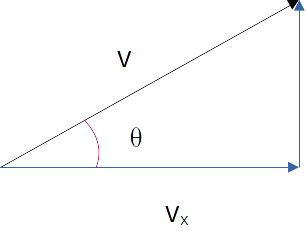
\includegraphics[scale=0.4]{Velocity_Angle.png}
\caption{A velocity that doesn't lie along one axis and be split into perpendicular components.}
\end{figure}

This means we can use the Pythagorean Theorem to find the final velocity.

\begin{equation}
v_f = \sqrt{v_{f,x}^2 + v_{f,y}^2}
\end{equation}

The direction of the final velocity can be given by the angle $\theta$, which is an angle relative to the $x$-direction. Since we have found the two legs of the triangle, we can use inverse tangent to find the angle.

\begin{equation}
\theta = tan^{-1} \, \left( \frac{v_{f,y}}{v_{f,x}} \right)
\end{equation}

\begin{exampleblock}

Two hockey players are skating perpendicularly toward the puck and collide. They get tangled up and slide along the ice together. The first player has a mass of $85.0 \, kg$ and approaches the puck along the $x$-axis at $8.00 \, \frac{m}{s}$. The second player has a mass of $100. \, \frac{m}{s}$ and approaches the puck along the $y$-axis at $6.00 \, \frac{m}{s}$. What is their velocity when tangled up after the collision (magnitude and direction)?

\begin{figure}[H]
\centering
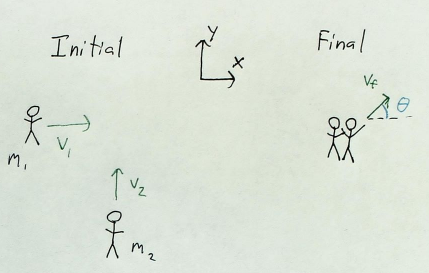
\includegraphics[scale=0.8]{hockey_collision.png}
\caption{Two hockey players collide when moving at a right angle. They get tangled up and slide together.}
\label{hockeycollision}
\end{figure}

\hspace{10pt}

Since the players get tangled up and slide together after the collision, this can be well modeled by a perfectly inelastic collision. Let's take stock of our known quantities. I will call the hockey player initially moving on the $x$-axis player 1, and the other player 2.

\begin{itemize}
\item $m_1 = 85.0 \, kg$
\item $v_{1,i,x} = 8.00 \, \frac{m}{s}$
\item $m_2 = 100. \, kg$
\item $v_{2,i,y} = 6.00 \, \frac{m}{s}$
\item $v_{1,i,y} = v_{2,i,x} = 0 \, \frac{m}{s}$
\end{itemize}

Now we can set up our $x$ and $y$ momentum conservation separately.

\begin{equation}
m_1 v_{1,i,x} = (m_1 + m_2) v_{f,x}
\end{equation}

\begin{equation}
m_2 v_{2,i,y} = (m_1 + m_2) v_{f,y}
\end{equation}

We can easily solve both of these to find the components of the final velocity.

\begin{equation}
v_{f,x} = \frac{m_1}{m_1 + m_2} v_{1,i,x} = \frac{85.0 \, kg}{85.0 \, kg + 100. \, kg} \cdot 8.00 \, \frac{m}{s} = 3.68 \, \frac{m}{s}
\end{equation}

\begin{equation}
v_{f,y} = \frac{m_2}{m_1 + m_2} v_{2,i,y} = \frac{100. \, kg}{85.0 \, kg + 100. \, kg} \cdot 6.00 \, \frac{m}{s} = 3.24 \, \frac{m}{s}
\end{equation}

The magnitude of their velocity is then

\begin{equation}
v_f = \sqrt{v_{f,x}^2 + v_{f,y}^2} = \sqrt{(3.68 \, \frac{m}{s})^2 + (3.24 \, \frac{m}{s})^2} = 4.90 \, \frac{m}{s}
\end{equation}

The direction relative to the $x$-axis is

\begin{equation}
\theta = tan^{-1} \, \left( \frac{v_{f,y}}{v_{f,x}} \right) = tan^{-1} \, \left( \frac{3.24 \, m/s}{3.68 \, m/s} \right) = 41.4^{\circ}
\end{equation}

\end{exampleblock}

\chapter{Rotational Motion}
\setcounter{example}{1}
\addtocounter{chp}{1}

So far most of the motion we have studied has been motion in a straight line or easily split into 2 perpendicular axes. This is what we call \textbf{linear motion}, where an object moves from one position to another.

In this chapter we will study \textbf{rotational motion}, which is motion along a circular path. We can actually do this by adapting the methods we used for linear motion to rotations.

\section{Variables of rotational motion}

We will first need to define quantities for rotational motion so that we can describe make a mathematical model of the motion. These quantities will all be \textit{rotational analogues} of linear motion, meaning that they have clear parallels in what we have already studied.

The rotational analogue of position is \textbf{angle}, which we will denote as $\theta$. Since rotational motion is motion around a circle it makes sense to think of position as an angle around the circle. For rotational motion we will measure angles in \textbf{radians}. As a reminder, a radian is the angle of a circle at which the portion of the circumference spanned is equal to the radius. You can see this in Figure \ref{radian}.

\begin{figure}[H]
\centering
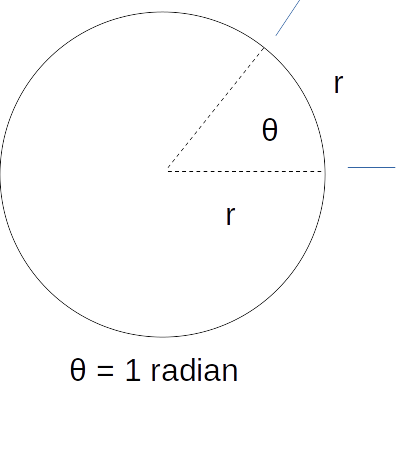
\includegraphics[scale=0.5]{radian_def.png}
\caption{One radian is the angle that spans a length along the circumference equal to the radius of the circle.}
\label{radian}
\end{figure}

Since the circumference of a circle is $C = 2 \pi r$, there are $2 \pi$ radians in a circle. This lets us convert between degrees and radians buy using

\begin{equation}
180^{\circ} = \pi \, rad
\end{equation}

One major difference we will see is in the units. Whereas position is a length measured in a unit of length (like the meter), angle does not have a unit of length. It is just given as an angle measured in radians.

Next we will introduce the rate of change in angle. This is the \textbf{angular velocity} and is denoted as $\omega$ (Greek letter lowercase omega). The average angular velocity is

\begin{equation}
\omega_{avg} = \frac{\Delta \theta}{\Delta t}
\end{equation}

The units of angular velocity are $s^{-1}$, which can also be written as $\frac{1}{s}$. This is a frequency, meaning how many times something happens per second. Here it is a measure of how many radians an object moves in 1 second.

\begin{exampleblock}

Suppose a merry-go-round completes completes 1 full revolution in 5.00 seconds. What is the average angular velocity of the merry-go-round?

\hspace{10pt}

There are $2 \pi$ radians in a full circle, so 1 revolution is an angle of $2 \pi$. This gives us $\Delta \theta = 2 \pi$ and $\Delta t = 5.00 \, s$. The average angular velocity is

\begin{equation}
\omega_{avg} = \frac{\Delta \theta}{\Delta t} = \frac{2 \pi}{5.00 \, s} = 0.400 \, \pi \, s^{-1}
\end{equation}

For rotational motion problems you can leave $\pi$ in your answer, as that makes the solution easier to understand. The angular velocity is $\omega_{avg} = 0.400 \, \pi \, s^{-1}$.

\end{exampleblock}

Our third quantity is the rate of change in angular velocity. This is the \textbf{angular acceleration} and is denoted as $\alpha$ (Greek letter lowercase alpha). The average angular acceleration is 

\begin{equation}
\alpha_{avg} = \frac{\Delta \omega}{\Delta t}
\end{equation}

The units of angular acceleration are $s^{-2}$, which can be written as $\frac{1}{s^2}$. This is the change in the frequency over time.

Sometimes we want to know the linear velocity of an object after we find the angular velocity so that we know how fast it is moving. First we will need to figure out the change in position from the change in angle. Remembering that a radian is the angle that gives a segment of the circumference equal to the radius, the actual position of an angle is the radius of the circle times the angle.

\begin{equation}
x = r \theta
\end{equation}

This means that 

\begin{equation}
v = \frac{\Delta x}{\Delta t} = \frac{r \Delta \theta}{\Delta t} = r \omega
\end{equation}

The magnitude of linear velocity is given by $v = r \omega$ and the direction is tangential to the circle. We can use a similar process to find the linear acceleration.

\begin{equation}
a = \frac{\Delta v}{\Delta t} = \frac{r \Delta \omega}{\Delta t} = r \alpha
\end{equation}

The magnitude of linear acceleration is given by $a = r \alpha$ and the direction is tangential to the circle.

\begin{exampleblock}

A race is just starting on a circular track. As the cars start, one car accelerates at $22.0 \, \frac{m}{s^2}$. If its angular acceleration is $0.629 \, s^{-2}$, what is the radius of the track?

\hspace{10pt}

We are given that $a = 22.0 \, \frac{m}{s^2}$ and $\alpha = 0.629 \, s^{-2}$. Now we can use the relationship between linear acceleration and angular acceleration.

\begin{equation}
a = r \alpha
\end{equation}

\begin{equation}
r = \frac{a}{\alpha} = \frac{22.0 \, m/s^2}{0.629 \, s^{-2}} = 35.0 \, m
\end{equation}

The radius of the track is $r = 35.0 \, m$.

\end{exampleblock}

\section{Positive/Negative and Right Hand Rule}

In linear motion we determined positive or negative values by setting a direction as positive at the start of the problem. How do we determine signs in rotational motion? It is actually very simple. An object can only rotate clockwise or counterclockwise around the circular path, so we need to define one direction as positive. The convention in physics is that \textbf{counterclockwise is positive}. We will follow this convention for all rotational motion problems that we study.



One related issue to sort out is assigning a vector direction to a quantity like angular velocity. The physical direction the object moves will be constantly changing, so we can't just have the vector aligned with the linear velocity of the object. To find a vector for angular velocity we will use the \textbf{right hand rule}.

Using your right hand, curl your fingers along the direction of rotation. Your thumb points in the direction of the vector for that rotational quantity. When drawn on paper, a positive angular velocity has a vector pointing out of the page. That is the positive direction for angular velocity. Figure \ref{rotvector} shows how we can draw vectors directed out of or into the page.


\begin{figure}[t]
\centering
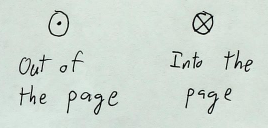
\includegraphics[scale=0.8]{vector_into_out.png}
\caption{How we draw vectors going into and out of the page. By convention in physics, out of the page (counterclockwise) is positive and into the page (clockwise) is negative}
\label{rotvector}
\end{figure}


The vector here is used to assign a clearly defined direction to a rotational quantity. We can see how the vector is defined in Figure \ref{omegavector}. This is used to keep track of direction with a vector, rather than trying to describe the plane and direction of rotation.

\begin{figure}[H]
\centering
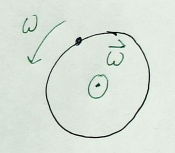
\includegraphics[scale=0.8]{omega_vector.png}
\caption{Right hand rule tells us that a counterclockwise angular velocity has its vector directed out of the page.}
\label{omegavector}
\end{figure}

\section{Rotational Kinematics}

If we have a constant angular acceleration, we can use the same kinematic equations as we did for linear motion but switch out the linear variables for their rotational analogues. Table \ref{kmrot} lists them below:

\begin{table}[H]
\large
\centering
\caption{Kinematic Equations for Rotations}
\label{kmrot}
\begin{tabular}{| c | c | c |}
	\hline
	Equation number & Formula & Missing variable \\
	\hline
	1 & $\omega_f = \omega_0 + \alpha t$ & No angle \\[5pt] \hline
	2 & $\Delta \theta = \frac{\omega_0 + \omega_f}{2} \cdot t$ & No angular acceleration \\[5pt] \hline
	3 & $\theta_f = \theta_0 + \omega_0 t + \frac{1}{2} \alpha t^2$ & No final angular velocity \\[5pt] \hline
	4 & $\omega_f^2 = \omega_0^2 + 2 \alpha \Delta \theta$ & No time \\[5pt]
	\hline
\end{tabular}
\end{table}

We can apply the exact same problem solving methods to rotational kinematics problems as we did with linear kinematics.

\begin{exampleblock}

A merry-go-round starts at rest and undergoes an angular acceleration until it reaches an angular velocity of $1.50 \, s^{-1}$. If the merry-go-round must rotate through an angle of $5.00 \, radians$, what is the angular acceleration of the merry-go-round?

\hspace{10pt}

First let's take stock of what we know.

\begin{itemize}
\item $\omega_0 = 0 \, s^{-1}$
\item $\omega_f = 1.50 \, s^{-1}$
\item $\Delta \theta = 5.00$
\end{itemize}

We want to find angular acceleration $\alpha$. We can do this most easily with kinematic equation 4.

\begin{equation}
\omega_f^2 = \omega_0^2 + 2 \alpha \Delta \theta
\end{equation}

\begin{equation}
\alpha = \frac{\omega_f^2 - \omega_0^2}{2 \Delta \theta} = \frac{(1.50 \, s^{-1})^2}{2 \cdot 5.00} = 0.225 \, s^{-2}
\end{equation}

The angular acceleration is $\alpha = 0.225 \, s^{-2}$

\end{exampleblock}

\section{Newton's 2nd Law in Rotations}

Now that we have our rotational quantities of motion, we can turn our attention to Newton's 2nd Law for rotations. For this we will need the rotational analogues of force and mass. 

First we will look at force. To understand this, you can do a little demonstration at home. Push a door open at the handle, then try pushing the same door open by pushing the door right near the hinges. You have to push much harder right near the hinge than at the handle in order to open the door. Why is that?

\begin{figure}[b]
\centering
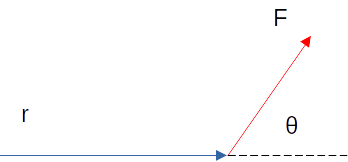
\includegraphics[scale=0.6]{torque_def.png}
\caption{Torque depends on the radius $r$ from the rotation axis, the magnitude of the force $F$, and the angle $\theta$ between $r$ and $F$.}
\label{torquedef}
\end{figure}

It is ``easier'' for a force to cause an angular acceleration when the force exerted further away from the rotation axis. The rotational analogue of force is \textbf{torque} and it is denoted $\tau$.

\begin{equation}
\overrightarrow{\tau} = \overrightarrow{r} x \overrightarrow{F} 
\end{equation}

The torque is the cross product of radius and force. The vector direction of the torque is perpendicular to both the radius and force. We won't go into too much detail on the vector operations here, but we can calculate the magnitude of the torque as

\begin{equation}
\tau = rF \, sin(\theta)
\end{equation}

where $\theta$ is the angle between the radius and force vectors (See Figure \ref{torquedef}). This means that the torque is maximized when the force is perpendicular to the radius. If the force is directed toward the axis of rotation, then $\theta = 0$ and the torque is zero. This makes sense that if we want to rotate an object we push around its pivot point, not straight at it!

Next we need the rotational analogue of mass. In linear motion mass determines an object's resistance to rotation, which is a property that we call inertia. We need to find an object's resistance to angular acceleration for the rotational analogue. That resistance depends not just on the mass, but also how the mass is distributed relative to the rotation axis. 

The resistance to angular acceleration is called the \textbf{moment of inertia} and is denoted $I$. If an object has more mass further from its rotation axis, that will increase the moment of inertia compared to having mass close to the axis. The moment of inertia for a given object depends on the shape of the object and the axis it is rotating around. Some commonly used moments of inertia are given in Table \ref{moi}.

\begin{table}[H]
\large
\centering
\caption{Common Moments of Inertia}
\label{moi}
\begin{tabular}{| c | c | c |}
	\hline
	Object (mass $m$) & Rotation Axis & Moment of Inertia \\
	\hline
	Point mass at radius $r$ & Center & $I = mr^2$ \\[5pt]
	\hline
	Hoop of radius $r$ & Center & $I = mr^2$ \\[5pt]
	\hline
	Uniform disk of radius $r$ & Center & $I = \frac{1}{2}mr^2$ \\[5pt]
	\hline
	Hollow sphere of radius $r$ & Center & $I = \frac{2}{3}mr^2$ \\[5pt]
	\hline
	Solid sphere of radius $r$ & Center & $I = \frac{2}{5} m r^2$ \\[5pt]
	\hline 
	Thin rod of length $L$ & Center & $I = \frac{1}{12} mr^2$ \\[5pt]
	\hline
	Thin rod of length $L$ & End of rod & $I = \frac{1}{3} mL^2$ \\[5pt]
	\hline
\end{tabular}
\end{table}

Notice how all of the moments of inertia have the form of mass times radius (or length) squared. The factor in front is due to the distribution of mass between the axis and the radius. See how the factor is larger for the hoop than the uniform disk. That is because the more mass is further away, the greater the moment of inertia is. 

The units of moment of inertia are $kg \cdot m^2$ and the units of torque are $N \cdot m$. Notice that the units of torque look just like the Joule, but torque is \textit{not} measured in Joules. It is a force acting at some length away from an axis, not a force acting over a distance.

\begin{exampleblock}

Find the moment of inertia of a golf club held at the grip end. To do this we will approximated the shaft as a thin rod and the clubhead as a point mass. The shaft has a mass of $60.0 \, g$ and is 1.06 $m$ long. The clubhead has a mass of $300. \, g$. What is the moment of inertia?

\hspace{10pt}

We are given the following:

\begin{itemize}
\item Mass of shaft $m_s = 60.0 \, g = 0.0600 \, kg$
\item Length of shaft $L = 1.06 \, m$
\item Mass of clubhead $m_c = 300. \, g = 0.300 \, kg$
\end{itemize}

We know the radius for the point mass clubhead is the length of the shaft, so we will use that in finding the moment of inertia for the clubhead. 

\begin{equation}
I_c = m_c L^2 = (0.300 \, kg) (1.06 \, m)^2 = 0.337 \, kg \cdot m^2
\end{equation}

The shaft is a thin rod rotating about one end, so

\begin{equation}
I_s = \frac{1}{3} m_s L^2 = \frac{1}{3} (0.060 \, kg) (1.06 \, m)^2 = 0.022 \, kg \cdot m^2
\end{equation}

Now we can find the total moment of inertia by adding up the two parts.

\begin{equation}
I = I_s + I_c = 0.359 \, kg \cdot m^2
\end{equation}

\end{exampleblock}

In the above example we see two things. The first is that we can approximate objects much smaller than their radius from rotation as point masses. The second is that we can find the moment of inertia of objects by splitting them into multiple parts and summing up the total at the end.

With our rotational analogues, Newton's 2nd Law gives us

\begin{equation}
\tau = I \alpha
\end{equation}

This lets us describe how interactions cause angular acceleration, just like how we previously used Newton's 2nd Law to describe how interactions cause linear acceleration.

\begin{exampleblock}

A solid disk of radius $25.0 \, cm$ is acted on its outer edge by a force of $4.00 \, N$ tangential to the edge of the disk. If the mass of the disk is $2.00 \, kg$, what is the angular acceleration of the disk?

\hspace{10pt}

The force is exerted at the outer edge of the disk, so the radius of the force is the same as the radius of the disk. This radius is $r = 25.0 \, cm = 0.250 \, m$. The disk mass is $m = 2.00 \, kg$ and the force is $F = 4.00 \, N$. Since the force acts tangential to the disk, $\theta = 90^{\circ}$. Look up the moment up inertia from Table \ref{moi}.

\begin{equation}
I = \frac{1}{2} m r^2
\end{equation}

The torque can be simplified since $sin(90^{\circ}) = 1$

\begin{equation}
\tau = rF \, sin(\theta) = rF
\end{equation}

Now we can use Newton's 2nd Law

\begin{equation}
\tau = I \alpha
\end{equation}

\begin{equation}
\alpha = \frac{\tau}{I} = \frac{rF}{mr^2} = \frac{F}{mr}
\end{equation}


\begin{equation}
\alpha = \frac{4.00 \, N}{(2.00 \, kg)(0.25 \, kg} = 8.00 \, s^{-2}
\end{equation}

The angular acceleration of the disk is $\alpha = 8.00 \, s^{-2}$.

\end{exampleblock}

\section{Work and Energy}

We can extend our rotational analogues to work and energy. This gives us an expression for work

\begin{equation}
W = \tau \, \Delta \theta
\end{equation}

Here we will use the signs of torque and change in angle to help us see if work should be positive or negative. If one is clockwise and the other counterclockwise, then the work will be negative. Otherwise the torque and motion are in the same direction and the work is positive.

Now for kinetic energy we get

\begin{equation}
KE = \frac{1}{2} I \omega^2
\end{equation}

Above is how we can find the kinetic energy of a rotating object.

\begin{exampleblock}

A bicycle wheel is spinning at an angular velocity of $15.0 \, s^{-1}$. Then a torque of $-0.450 \, N \cdot m$ is exerted on the wheel while it rotates through 2 revolutions so that it slows down. The wheel can be approximated as a hoop of mass $0.350 \, kg$ and radius $0.400 \, m$. What is the final angular velocity of the wheel?

\hspace{10pt}

Let's take stock of what we know

\begin{itemize}
\item $\omega_i = 15.0 \, s^{-1}$
\item $\tau = -0.450 \, N \cdot m$
\item $m = 0.350 \, kg$
\item $r = 0.400 \, m$
\item $\Delta \theta = 4 \pi$
\end{itemize}

We want to solve for $\omega_f$. This is a hoop, so the moment of inertia is $I = mr^2$. We can use the work-kinetic energy theorem.

\begin{equation}
W = \Delta KE = KE_f - KE_i
\end{equation}

\begin{equation}
\tau \, \Delta \theta = \frac{1}{2} I \omega_f^2 - \frac{1}{2} I \omega_i^2
\end{equation}

\begin{equation}
\frac{2 \tau \, \Delta \theta}{I} = \omega_f^2 - \omega_i^2
\end{equation}

\begin{equation}
\omega_f^2 = \frac{2 \tau \, \Delta \theta}{mr^2} + \omega_i^2
\end{equation}

\begin{equation}
\omega_f = \sqrt{ \frac{2 \tau \, \Delta \theta}{mr^2} + \omega_i^2}
\end{equation}

\begin{equation}
\omega_f = \sqrt{ \frac{2 (-0.450 \, N \cdot m) (4 \pi)}{(0.350 \, kg)(0.400 \, m)^2} - (15.0 \, s^{-1})^2} = 4.80 \, s^{-1}
\end{equation}

The final angular velocity is $\omega_f = 4.80 \, s^{-1}$.

\end{exampleblock}

\section{Rolling}

We can combine linear and rotational motion in rolling. For this text, we will specifically study \textbf{rolling without slipping or sliding}. That means that it rolls smoothly and never slides on the surface or ``spins out'' without moving. 

Suppose that we have an object that is rolling with an angular velocity $\omega$. We want to relate the linear velocity of the wheel, which we will call the center of mass velocity ($v_{CoM}$) to the angular velocity of the wheel. From our definition of rotational quantities, remember that we can relate the angular velocity to the linear velocity at the outer edge of the rolling object as

\begin{equation}
v = r \omega
\end{equation}

The condition that the object doesn't slip or slide tells us something very import about the motion: \textit{the bottom of the object that is in contact with the surface is stationary relative to the surface.} That means the linear velocity of the center of mass of the object is the same as the linear velocity of the outer edge of the object.

\begin{equation}
v_{CoM} = r \omega
\end{equation}

With this we can relate the linear velocity of a rolling object to its angular velocity. With this we can look at the kinetic energy of a rolling object.

\begin{equation}
KE = \frac{1}{2} m v_{CoM}^2 + \frac{1}{2} I \omega^2
\end{equation}

We can write this exclusively in terms of either $\omega$ or $v_{CoM}$. Below we will show this for $v_{CoM}$.

\begin{equation}
KE = \frac{1}{2} m v_{CoM}^2 + \frac{1}{2} I \frac{v_{CoM}^2}{r^2}
\end{equation}

\begin{exampleblock}

A ball bearing (solid sphere) is launched from a spring. It starts at rest and is compressed $1.20 \, cm$ on a spring with spring constant $k = 20.0 \, \frac{N}{cm}$. The ball bearing has mass $25.0 \, g$ and radius $r = 1.00 \, cm$. What is the center of mass velocity of the ball bearing after it is launched? (Use conservation of energy to approach this problem.)

\hspace{10pt}

Let's take stock of our known values

\begin{itemize}
\item $\Delta x_i = 1.20 \, cm = 0.0120 \, m$ (Compression of spring)
\item $k = 20.0 \, \frac{N}{cm} = 2000 \, \frac{N}{m}$
\item $m = 25.0 \, g = 0.0250 \, kg$
\item $r = 1.00 \, cm = 0.0100 \, m$
\end{itemize}

Since it starts at rest, there is no kinetic energy in the initial state. We want to find the center of mass velocity in the final state, $v_{CoM,f}$. Final state is just kinetic energy. 

\begin{itemize}
\item $PE_i = \frac{1}{2} k (\Delta x_i)^2$
\item $KE_f = \frac{1}{2} m v_{CoM,f}^2 + \frac{1}{2} I \omega_f^2$
\item $KE_i = PE_f = 0 \, J$
\end{itemize}

Now we can use conservation of energy and substitute $\omega_f = \frac{v_{CoM,f}}{r}$

\begin{equation}
\frac{1}{2} k (\Delta x_i)^2 = \frac{1}{2} m v_{CoM,f}^2 + \frac{1}{2} I \frac{v_{CoM,f}^2}{r^2}
\end{equation}

Now we need to use Table \ref{moi} for the moment of inertia of the ball bearing $I = \frac{2}{5} m r^2$.

\begin{equation}
k (\Delta x_i)^2 = m v_{CoM,f}^2 + \frac{2}{5} m r^2 \frac{v_{CoM,f}^2}{r^2}
\end{equation}

The radius cancels out of the second term on the right hand side! We will keep simplifying.

\begin{equation}
k (\Delta x_i)^2 = m v_{CoM,f}^2 \left(1 + \frac{2}{5} \right)
\end{equation}


\begin{equation}
k (\Delta x_i)^2 = \frac{7}{5} m v_{CoM,f}^2
\end{equation}

\begin{equation}
v_{CoM,f}^2 = \frac{5 k (\Delta x_i)^2}{7 m}
\end{equation}

\begin{equation}
v_{CoM,f} = \sqrt{\frac{5 k (\Delta x_i)^2}{7 m}}
\end{equation}

\begin{equation}
v_{CoM,f} = \sqrt{\frac{5 (2000 \, N/m)(0.0120 \, m)^2}{7 (0.0250)}} = 2.87 \, \frac{m}{s}
\end{equation}

The center of mass velocity of the ball bearing is $v_{CoM,f} = 2.87 \, \frac{m}{s}$

\end{exampleblock}

This is slower than if we were to launch a block of the same mass that slides because some kinetic energy goes into the rotation rather than the center of mass velocity.

\section{Angular Momentum}

Perhaps unsurprisingly, there is also a rotational analogue of momentum called \textbf{angular momentum}. Angular momentum is denoted with an $L$ and is found by

\begin{equation}
L = I \omega
\end{equation}

It is the moment of inertia times angular velocity, similar to linear momentum being the mass times velocity. Similar to conservation of momentum, \textbf{angular momentum is conserved whenever there is no external torque}.

\begin{equation}
L_i = L_f
\end{equation}

\begin{equation}
I_i \omega_i = I_f \omega_f
\end{equation}

For a real world example, this is why ice skaters can increase their angular velocity by tucking their arms up to their torso. Pulling their arms in reduces their moment of inertia, which means their angular velocity must increase in order to conserve angular momentum.

\begin{exampleblock}

Carrie is on a playground merry-go-round. The merry-go-round is a uniform solid disk of mass $180 \, kg$ and radius $1.5 \, m$. Carrie has a mass of $35.0 \, kg$. She is initially at the outer edge of the merry-go-round when it is rotating with an angular velocity of $2.00 \, s^{-1}$. She then moves halfway toward the center of the merry-go-round. Treating Carrie as a point mass, use conservation of angular momentum to find the new angular velocity of the merry-go-round.

\hspace{10pt}

Carrie starts out at the full radius of the merry-go-round in the initial state, and moves to half the radius for the final state. We will take stock of our known values. I will use subscript $d$ for the merry-go-round disk and subscript $c$ for Carrie.

\begin{itemize}
\item $m_d = 180 \, kg$
\item $m_c = 35.0 \, kg$
\item $r_d = 1.5 \, m$
\item $r_{c,i} = r_d = 1.5 \, m$
\item $r_{c,f} = \frac{1}{2} r_d = 0.75 \, m$
\item $\omega_i = 2.00 \, s^{-1}$
\end{itemize}

The moment of inertia of the disk stays constant while Carrie's changes. Let's use conservation of angular momentum.

\begin{equation}
I_i \omega_i = I_f \omega_f
\end{equation}

\begin{equation}
(I_d  + I_{c,i}) \omega_i = (I_d + I_{c,f}) \omega_f
\end{equation}

\begin{equation}
\omega_f = \frac{I_d + I_{c,i}}{I_d + I_{c,f}} \omega_i
\end{equation}

\begin{equation}
I_d = \frac{1}{2} m_d r_d^2 = \frac{1}{2} (180 \, kg) (1.5 \, m)^2 = 202.5 \, kg \cdot m^2
\end{equation}

Now we can find Carrie's moment of inertia in both the initial and final state.

\begin{equation}
I_{c,i} = m_c r_{c,i}^2 = (35.0 \, kg)(1.5 \, m)^2 = 78.75 \, kg \cdot m^2
\end{equation}

\begin{equation}
I_{c,f} = m_c r_{c,f}^2 = (35.0 \, kg)(0.75 \, m) = 19.69 \, kg \cdot m^2
\end{equation}

When we plug these in we get

\begin{equation}
\omega_f = 2.53 \, s^{-1}
\end{equation}

The final angular velocity is $\omega_f = 2.53 \, s^{-1}$.

\end{exampleblock}

\chapter{The Solar System}
Now we will take a little detour away from the surface of the Earth and look at the solar system. Newton made tremendous contributions to our understanding of the dynamics of the solar system. To see why, first we must look back at the history of humanity's study of the solar system.

Throughout history, we can see a variety of explanations for the existence of the Sun, Moon, planets, and stars. Sometimes this was tied to a creation myth, with the Sun and other ``heavenly'' bodies being gods. We will focus on efforts to model and explain the motion of the solar system bodies and stars.

\section{Geocentric Model}

An early model that is strongly associated with Greek thinkers is the \textbf{geocentric} model. This model had the Earth at the center of the solar system with the Sun, Moon, other planets, and stars (known collectively as the \textbf{celestial bodies}) orbiting around the Earth. This seems like a natural starting point for models because all objects we see in the sky move across the sky in a way that appears as though they are moving around the Earth.

The Greek model featured a series of concentric (same center) spherical shells around the Earth. The celestial bodies each had their own shells for their individual orbits around the Earth. The outermost shells were the fixed stars, called such because they did not move relative to each other while the other bodies moved relative to the stars.

One issue that stumped Greek astronomers was the \textbf{retrograde motion} of the planets. This is when a planet appears to move ``backward'' across the sky for a period of several weeks before continuing its normal motion. The basic spherical shell geocentric model had no explanation for this. The solution that emerged was to add \textbf{epicycles} to the circular orbits of the planets. Epicycles were small circles along the circular orbit on which the planet moved and explained retrograde motion by allowing the planet to move in the opposite direction for a time. This model is accredited largely to the Greek thinker Ptolemy, and is known as the Ptolemaic model. The addition of epicycles did not fix all the issues with the motion of planets, so it ended up with epicycles upon epicycles! Figure \ref{geocentric} shows an illustration of the Ptolemaic model.

\begin{figure}[t]
\centering
\includegraphics[scale=0.4]{geocentric.jpg}
\caption{An illustration of Ptolemy's geocentric model made Bartolomeu Velho in 1568. You can see each planet has a shell, plus separate shells for the Sun and Moon.}
\label{geocentric}
\end{figure}

Ptolemy's geocentric model of circular orbits with epicycles was the accepted model of the solar system among European academics for over 1000 years. In large part this was due to the Catholic Church adopting this model as part of their doctrine. Studying or teaching other models came with a risk to one's academic career or even personal freedom.

\section{Heliocentric Model}

The next major advancement in modeling the solar system was the \textbf{heliocentric} model. As the name implies, this model has the Sun at the center of the solar system. All of the planets, including Earth, orbit around the Sun in perfect circles. The advancement of a heliocentric model is largely credited to Nicolaus Copernicus. He was not the first person to develop a heliocentric model but his work was what took hold. He had it published shortly before his death, avoiding any controversy that his model would cause.

Copernicus explained the retrograde motion as a consequence of our perspective from Earth and the varying speeds of each planet in their orbits. However, he was unable to accurately model the positions of the planets across the sky, so he did need to add some epicycles to the model.

\section{Kepler's Laws of Planetary Motion}

Improving upon Copernicus's model required more precise observations than had been previously undertaken. Fortunately, Tycho Brahe was taking exactly the observations required. Telescopes were not available to him, so he made is observations with the naked eye using a small slit in the wall to accurately track the position on the sky a planet was seen on a given night. Since Galileo developed his telescope shortly after Tycho took his measurements, they stand as the most precise naked eye astronomical measurements ever taken. Tycho unfortunately passed away before his observations could be used to improve models of the solar system, so his assistant Johannes Kepler took over this work.

Kepler used the incredibly precise observations that Tycho took and got to work on figuring out what was wrong in the existing heliocentric models. This work culminated in Kepler's Laws of Planetary Motion.

\linespace

Kepler's 1st Law of Planetary Motion states that

\hspace{10pt}

\textbf{The motion of each planet around the Sun is an ellipse with the Sun at one focus}

\linespace

Compared to Copernicus's model, this is a major change. Historically, circles were often the modeled orbit because the motion of the heavens was thought to be perfect, and therefore should have perfect circles. Kepler used Tycho's data and found that the only way to fit his observations was for the orbits to be elliptical instead of circular. This eliminated the need to add epicycles to accurately model the positions of the planets.

\begin{figure}[H]
\centering
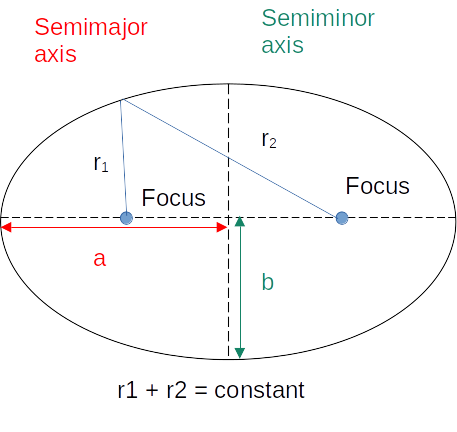
\includegraphics[scale=0.8]{EllipseDef.png}
\caption{Definition of an ellipse. It is a shape where the sum of the distances of the curve from the two foci is constant. In the solar system, the Sun is at one focus of the orbit.}
\label{ellipsedef}
\end{figure}

Figure \ref{ellipsedef} shows the definition of an ellipse. The ellipse is defined using the length from focus 1, $r_1$, and focus 2, $r_2$. The sum of those lengths is constant.

\begin{equation}
r_1 + r_2 = constant
\end{equation}

Kepler's 1st Law of Planetary motion tells us the Sun as at one of the foci. Later on, we will use the semimajor axis $a$, so remember that it is half of the long dimension of the ellipse.

\linespace

Kepler's 2nd Law of Planetary Motion states that

\textbf{A line from the Sun to a planet sweeps an equal area in equal time during its orbit.}

\linespace

The statement of Kepler's 2nd Law of Planetary motion is short but might be unclear. Figure \ref{Keplers2nd} shows a visual of this. We see two different 30 days intervals of a planet's orbit. The two triangles (at least nearly triangles) formed have the same area since they are an equal time in orbit. We see that for the area to be the same, the planet must move further when it is closer to the Sun. Since the time interval is the same, the planet moves faster when it is closer to the Sun.

\begin{figure}[H]
\centering
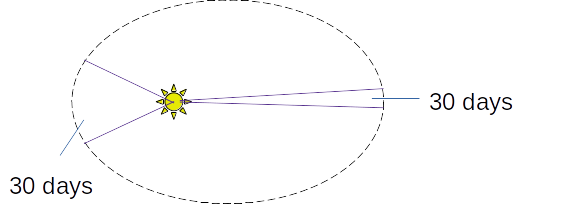
\includegraphics[scale=0.6]{Keplers2nd.png}
\caption{We see the line connecting the Sun to a planet over two different 30 day intervals. To have the same area, the planet must move further along its orbit when it is closer to the Sun. Moving further in the same time interval means that it must be moving faster. (Note that the ellipse of the orbit is exaggerated compared to the planets in our solar system.)}
\label{Keplers2nd}
\end{figure}

\linespace 

Kepler's 3rd Law of planetary motion states that

\hspace{10pt}

\textbf{For all planets orbiting the Sun, the square of the orbital period is proportional to the cube of the semimajor axis.}

\linespace

\textbf{Orbital period} is the time it takes for a planet to complete one orbit around the Sun. Semimajor axis is a physical length from the ellipse of the orbit. For nearly circular orbits like the planets in the solar system, this is roughly equal to the distance from the Sun to the planet. You can think of it like an ``orbital radius'', just remember it is not a fixed radius.

We get a useful mathematical relationship from Kepler's 3rd Law of Planetary Motion. For the orbital period $T$ and semimajor axis $a$ we have

\begin{equation}
T^2 \propto a^3
\end{equation}

There is a constant of proportionality, but we don't necessarily know that. We can rewrite this as

\begin{equation}
\frac{T^2}{a^3} = constant
\end{equation}

where this ratio is constant for all planets in the solar system. In fact, this ratio is constant for every object that orbits the Sun. Since this ratio is constant throughout the solar system, we can compare two planets using

\begin{equation}
\frac{T_1^2}{a_1^3} = \frac{T_2^2}{a_2^3}
\end{equation}

If we know both the orbital period and semimajor axis for one planet, we can find an unknown quantity from another planet or other body in the solar system.

\section{Using Kepler's 3rd Law in the Solar System}

Now that we have Kepler's 3rd Law, how can we use it to study the solar system? We can start with the Earth and find the ratio $\frac{T^2}{a^3}$. This ratio will be constant for every other body that orbits the Sun.

Choosing proper units will make this much easier to do. For the orbital period, we will use years. Since a year is defined as the orbital period of the Earth, we have

\begin{equation}
T_{Earth} = 1 \, year
\end{equation} 

For the semimajor axis, we will want to choose appropriate length units. To put the size of the solar system into perspective, the average Earth-Sun distance is $1.5 \cdot 10^{11} \, m$. That is 150 \textbf{billion} meters! Rather than work with numbers that large, it is easier to define a new unit that better suits the scale of the problem. The \textbf{astronomical unit} is defined as the average Earth-Sun distance. It is abbreviated as $AU$ and defined as

\begin{equation}
1 \, AU = 1.5 \cdot 10^{11} \, m
\end{equation}

Since the Earth's orbit is nearly circular, the semimajor axis is very nearly the same as the average Earth-Sun distance.

\begin{equation}
a_{Earth} = 1 \, AU
\end{equation}

That means that when we measure the orbital period in years and semimajor axis in astronomical units, the ratio from Kepler's 3rd Law for the Earth is

\begin{equation}
\frac{T^2}{a^3} = 1
\end{equation}

For these units, every body in the solar system has a ratio of 1. Once either the orbital period or semimajor axis is known, the other can be solved for.

\begin{exampleblock}

Jupiter has an orbital period of 11.9 years. What is the semimajor axis of its orbit?

\hspace{10pt}

If we measure our semimajor axis in $AU$, we will have

\begin{equation}
\frac{T^2}{a^3} = 1
\end{equation}

\begin{equation}
a^3 = T^2
\end{equation}

\begin{equation}
a = T^{2/3} = 11.9^{2/3} = 5.2 \, years
\end{equation}

Jupiter's orbital period is $T = 5.2 \, years$.

\end{exampleblock}

\section{Newton's Law of Universal Gravitation}

Kepler accurately described the motion of the planets, but he did not explain \textit{why} the planets orbit the Sun as described by his 3 laws. That explanation would have to wait for Isaac Newton and his \textbf{Law of Universal Gravitation}. Any two objects with mass exert an attractive gravitational force on each other, each pulling on the other. For two objects with masses $m_1$ and $m_2$ separated by a distance $r$, the gravitational force between them is

\begin{equation}
F_g = \frac{-G m_1 m_2}{r^2}
\end{equation}

The negative sign indicates the force is attractive, which is a convention that you will see in electricity and magnetism if you continue your studies in physics. The capital $G$ is the \textbf{gravitational constant}

\begin{equation}
G = 6.67 \cdot 10^{-11} \, \frac{m^3}{kg \, s^2}
\end{equation}

Remember that this is different from lowercase $g$, which is the gravitational acceleration at the Earth's surface. The gravitational constant is a fundamental constant of the universe that was measured through careful experiments.

\begin{exampleblock}

Anthony and Bennett are sitting 2.00 meters apart. If Anthony's mass is $75.0 \, kg$ and Bennett's mass is $68.0 \, kg$, what is the magnitude of the gravitational force between them?

\hspace{10pt}

Let's take stock of our known quantities

\begin{itemize}
\item $r = 2.00 \, m$
\item $m_A = 75.0 \, kg$
\item $m_B = 68.0 \, kg$
\end{itemize}

The force of gravity between them is

\begin{equation}
F_g = \frac{-G m_A m_B}{r^2}
\end{equation}

\begin{equation}
F_g = \frac{-(6.67 \cdot 10^{-11} \, m^3 \, kg^{-1} \, s^{-2}) (75.0 \, kg) (68.0 \, kg)}{(2.00 \, m)^2} = -8.50 \cdot 10^{-8} \, N
\end{equation}

The magnitude of the force between them is $|F_g| = 8.50 \cdot 10^{-8} \, N$. Gravitational forces between a person and anything other than the Earth can be safely ignored in modeling motion!
\end{exampleblock}

With Newton's Laws of Motion and Newton's Law of Universal Gravitation, physics had a consistent framework to model motion on the Earth's surface and in space. Before Newton, motion on Earth and motion of the ``heavenly'' bodies were thought to be completely separate. Except for motion approaching the speed of light (which is $3.00 \cdot 10^8 \, \frac{m}{s}$) or in very strong gravitational fields (like near black holes), the problem solving techniques in this text can be applied to motion in space!

\section{Orbit of the Moon}

The Moon is Earth's lone natural satellite. You are likely familiar with satellites meaning man-made objects put into orbit around the Earth. Natural satellites refers to moons around a planet. Mercury and Venus have no moons while the gas giants have dozens of moons each. The Earth's Moon was likely created by a large (possibly Mars-sized) body striking the Earth and ejecting a large amount of material into space, which later came together under the attraction of gravity to form the Moon. 

The orbital period of the Moon is 27.3 days, so roughly 1 month. Figure \ref{phases} shows how this causes us to see the different \textbf{phases of the Moon}. Half of the Moon is always illuminated by the Sun, but how much of that illuminated side we see changes throughout the month. Nothing is changing about the Moon, just a change in the relative positions of the Sun-Earth-Moon system.

\begin{figure}[H]
\centering
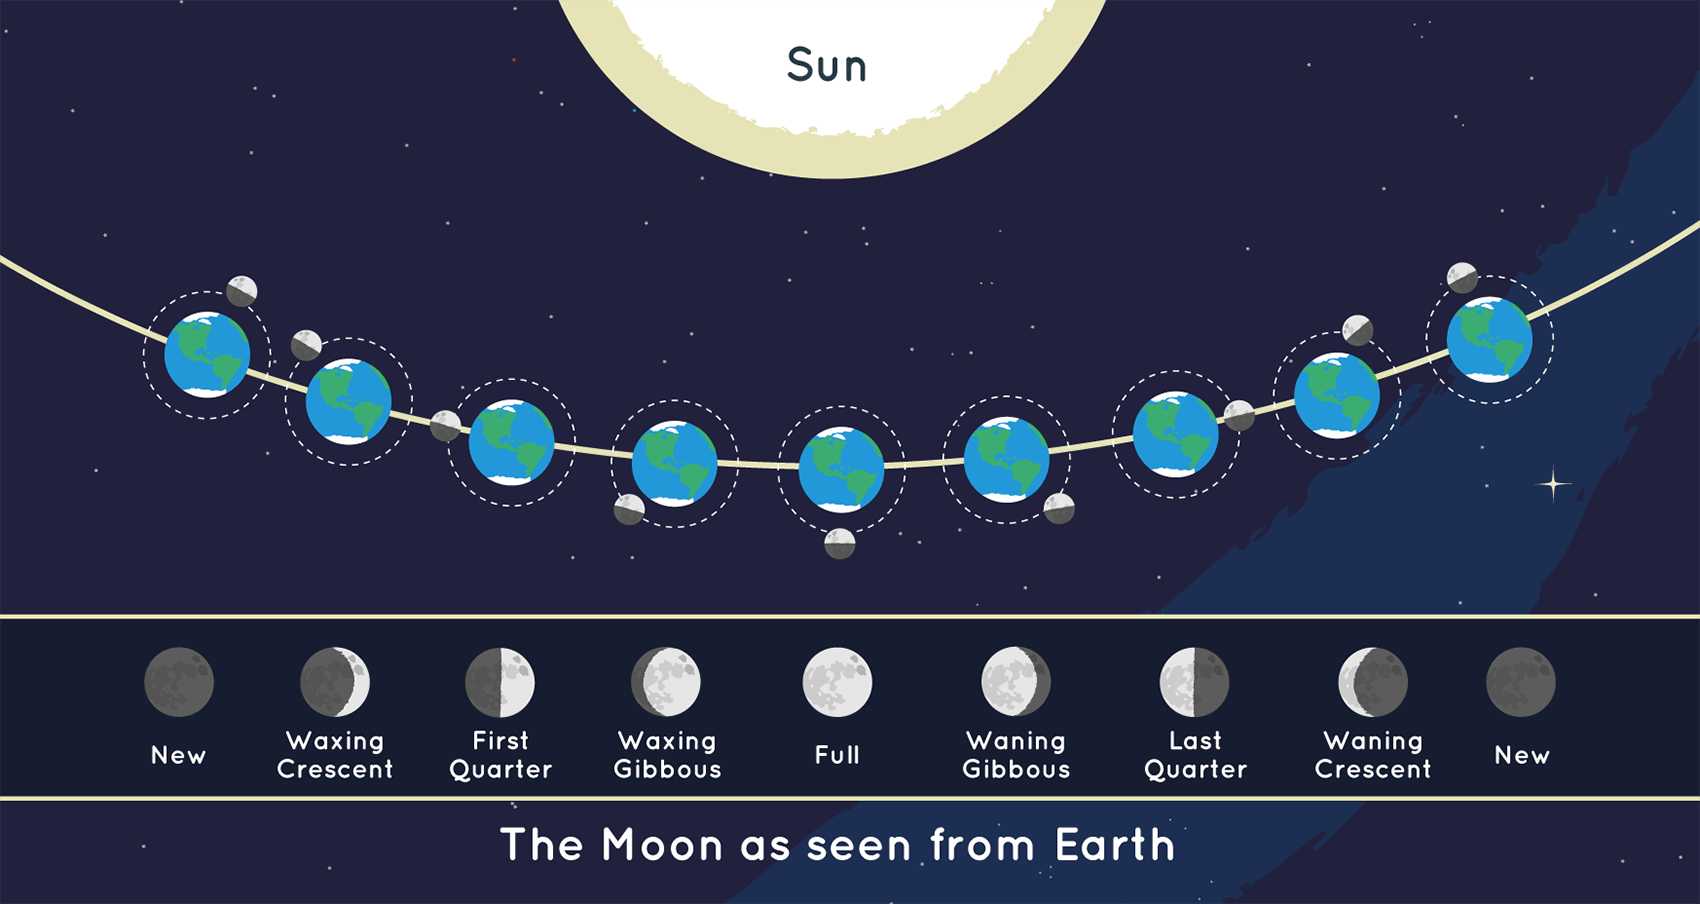
\includegraphics[scale=0.23]{359_moon-phases-jpl.png}
\caption{The phases of the Moon are caused by the Moon's orbit around the Earth and our perspective from the Earth. \textit{Image Credit: NASA/JPL-Caltech}}
\label{phases}
\end{figure}

As the Moon orbits the Earth, the same side of the moon always faces the Earth because the rotation period of the Moon is the same as the orbital period. This is a phenomenon known as \textbf{tidal locking} and is caused by the difference in gravitational force exerted on the near and far side of the Moon. Astronomers have found planets around other stars (called extra-solar planets) that are tidally locked. Many of the moons around other planets in the solar system are also tidally locked with their planet.

The moon being tidally locked is what leads to the slightly misnamed dark side of the Moon, which is the side that always faces away from Earth. Think of dark as meaning ``unknown'' instead of ``no light''. It is also (and more accurately in my opinion) known as the far side of the Moon

Figure \ref{phases} also shows why the moon rises and sets at different times of day throughout the month. Only in the full moon phase is the Moon directly overhead 12 hours after the sun (roughly midnight). You likely have seen the moon during daytime during the quarter or crescent phases. This is because of where the Moon is relative to the sun and the Earth for that fraction of the illuminated half of the Moon to be visible from Earth.

\section{Eclipses}



\end{document}
